% Retoca las líneas marcadas con TODO según las necesidades

\documentclass[oneside,a4paper,12pt]{book} % TODO: cambia "oneside" por "twoside" a la hora de imprimirlo

\usepackage[spanish]{babel}
\usepackage[utf8]{inputenc}
\usepackage{geometry}
\usepackage{makeidx}
\usepackage{url}
\usepackage{graphicx}
\usepackage{color}
\usepackage{caption}
\usepackage{acronym}
\usepackage{hyphenat}
\usepackage{a4wide}
\usepackage[normalsize]{subfigure}
\usepackage{float}
\usepackage{titlesec}
\usepackage{multirow}
\usepackage{tabularx}
\usepackage{array}
\usepackage[Lenny]{fncychap}
\usepackage{listings} % para poder hacer uso de "listings" propios (p.ej. códigos)
\usepackage{eurosym} % para poder usar el símbolo del euro con \euro {xx}
\usepackage{hyperref} % TODO: añade la opción hidelinks para imprimirlo (los enlaces no aparecerán resaltados)

% Para que no parta las palabras
%pretolerance=10000

\newcommand{\bigrule}{\titlerule[0.5mm]} \titleformat{\chapter}[display] % cambiamos el formato de los capítulos
{\bfseries\Huge} % por defecto se usaron caracteres de tamaño huge en negrita
{% contenido de la etiqueta 
\titlerule % línea horizontal 
\filright % texto alineado a la derecha 
\Large\chaptertitlename\ % capítulo e índice en tamaño large
\Large % en lugar de 
\Huge \Large\thechapter} 
{0mm} % espacio mínimo entre etiqueta y cuerpo
{\filright} % texto del cuerpo alineado a la derecha
[\vspace{0.5mm} \bigrule] % después del cuerpo, dejar espacio vertical y trazar línea horizontal gruesa
\geometry{a4paper, left=3.5cm, right=2cm, top=3cm, bottom=2cm, headsep=1.5cm}

% Estilos para ilustrar códigos:
\definecolor{code_green}{rgb}{0,0.6,0}
\definecolor{code_gray}{rgb}{0.5,0.5,0.5}
\definecolor{code_mauve}{rgb}{0.58,0,0.82}

\lstset{frame=tb,
  language=C,
  aboveskip=3mm,
  belowskip=3mm,
  showstringspaces=false,
  columns=flexible,
  basicstyle={\small\ttfamily},
  numbers=none,
  numberstyle=\tiny\color{code_gray},
  keywordstyle=\color{blue},
  commentstyle=\color{code_green},
  stringstyle=\color{code_mauve},
  breaklines=true,
  breakatwhitespace=true,
  tabsize=3
}

\lstset{frame=tb,
  language=C++,
  aboveskip=3mm,
  belowskip=3mm,
  showstringspaces=false,
  columns=flexible,
  basicstyle={\small\ttfamily},
  numbers=none,
  numberstyle=\tiny\color{code_gray},
  keywordstyle=\color{blue},
  commentstyle=\color{code_green},
  stringstyle=\color{code_mauve},
  breaklines=true,
  breakatwhitespace=true,
  tabsize=3
}

\lstset{frame=tb,
  language=Python,
  aboveskip=3mm,
  belowskip=3mm,
  showstringspaces=false,
  columns=flexible,
  basicstyle={\small\ttfamily},
  numbers=none,
  numberstyle=\tiny\color{code_gray},
  keywordstyle=\color{blue},
  commentstyle=\color{code_green},
  stringstyle=\color{code_mauve},
  breaklines=true,
  breakatwhitespace=true,
  tabsize=3
}

% Definición de mis propios tipos: Códigos, Ecuaciones y Tablas
\DeclareCaptionType{code}[Código][Listado de códigos]
\DeclareCaptionType{myequation}[Ecuación][Listado de ecuaciones]

% TODO: especifica las reglas de separación que consideres. Algunos ejemplos:
\hyphenation{fuer-tes}
\hyphenation{mul-ti-ca-pa}
\hyphenation{res-pues-ta}
\hyphenation{di-fe-ren-tes}
\hyphenation{de-sa-rro-lla-dos}
\hyphenation{re-pre-sen-tan-do}

 % archivo de configuraci�n de estilo

\makeindex

\begin{document}
\baselineskip 1.35\baselineskip

\frontmatter

\thispagestyle{empty}
\vspace{2cm}

\begin{figure}[htb]
  \centerline{\resizebox{.60\textwidth}{!}{
\includegraphics{figs/logo_urjc}}}
\end{figure}

\begin{center}
  {\Large {\bf GRADO EN INGENIERÍA DE TECNOLOGÍAS INDUSTRIALES}}
  \vspace{5mm}
 
  {\large {Escuela Superior de Ciencias Experimentales y Tecnología}}
  \vspace{5mm}

  {\large {Curso académico 2023-2024}}

  \vspace{1cm}

  {\large {\bf Trabajo Fin de Grado}}

  \vspace{2cm}

  {\Large {Escribe el título del trabajo aquí\\
               con la segunda línea aquí\\[1cm] }}

  \vspace{5cm}
  {\bf Tutor}: Julio Vega Pérez \\
  {\bf Autor}: David Campoamor Medrano
\end{center}

\clearpage
\thispagestyle{empty}


% Este diseño se corresponde con la licencia CC-BY-NC-SA.
% Por supuesto, puedes poner la licencia que mejor se adapte al propósito de tu trabajo.
% Recuerda que, si no se especifica ninguna licencia, esta -como cualquier creación artística- pasaría a estar licenciada con todos los derechos reservados (copyright).


\thispagestyle{empty}
\begin{center}
    
\includegraphics[width=0.45\textwidth]{figs/logo_urjc.jpg}\\[1cm]

    {\large{\textbf{Grado en Ingeniería de Tecnologías Industriales}}}\\[1cm]
    {\large{\textbf{Trabajo de Fin de Grado}}}\\[1cm]
\end{center}


El presente trabajo, titulado \textit{\textbf{SISTEMA DE RECOLECCIÓN ROBÓTICO DE FRESAS MADURAS POR VISIÓN ARTIFICIAL}}, constituye la memoria correspondiente a la asignatura Trabajo de Fin de Grado que presenta D./D\textsuperscript{a}. \textit{\textbf{DAVID CAMPOAMOR MEDRANO}} como parte de su formación para aspirar al Título de Graduado/a en Ingeniería de Tecnologías Industriales. Este trabajo ha sido realizado en la \textit{\textbf{ESCUELA DE INGENIERÍA DE FUENLABRADA}} en el \textit{\textbf{DEPARTAMENTO DE TEORÍA DE LA SEÑAL Y COMUNICACIONES Y SISTEMAS TELEMÁTICOS Y COMPUTACIÓN}} bajo la dirección de \textit{\textbf{JULIO VEGA PÉREZ}}.\\[3cm]

\begin{flushright}
Móstoles, 26 de mayo de 2025
\end{flushright}

\cleardoublepage

\begin{figure}
 \ \ \ \ 
\includegraphics[width=0.25\linewidth]{figs/by-nc-sa.png}
 \label{fig:cc} 
 \end{figure}

\

\

\

\noindent
Este trabajo se distribuye bajo los términos de la licencia internacional \href{http://creativecommons.org/licenses/by-nc-sa/4.0/}{CC BY-NC-SA International License} (Creative Commons AttributionNonCommercial-ShareAlike 4.0). Usted es libre de \textit{(a) compartir}: copiar y redistribuir el material en cualquier medio o formato; y \textit{(b) adaptar}: remezclar, transformar y crear a partir del material. El licenciador no puede revocar estas libertades mientras cumpla con los términos de la licencia:

\begin{itemize}
\item \textit{Atribución}. Usted debe dar crédito de manera adecuada, brindar un enlace a la licencia, e indicar si se han realizado cambios. Puede hacerlo en cualquier forma razonable, pero no de forma tal que sugiera que usted o su uso tienen el apoyo de la licenciante.
\item \textit{No comercial}. Usted no puede hacer uso del material con propósitos comerciales.
\item \textit{Compartir igual}. Si remezcla, transforma o crea a partir del material, debe distribuir su contribución bajo la la misma licencia del original.
\end{itemize}

\begin{flushright}
		\vspace{7.0 cm}
		\emph{Documento de} \textbf{David Campoamor Medrano}. % TODO: pon aquí tu nombre cuando hagas el documento
\end{flushright}



\cleardoublepage

\chapter*{Agradecimientos}

Nunca es tarea fácil agradecer a tantas personas el apoyo, la ayuda y los consejos que han contribuido en mi beneficio, tanto personal como académico, durante todos estos años.\\

En primer lugar, me gustaría dar las gracias tanto a la Universidad Rey Juan Carlos como a todos los profesores de los que he tenido el privilegio de ser alumno, por haber sido capaces de transmitir la dedicación, pasión, disciplina y el esfuerzo tan imprescindible como necesarios para la praxis de una profesión como lo es la de ingeniero, y más concretamente en mi caso, la de ingeniero industrial.\\
Quisiera expresar mi gratitud a mi tutor, Julio Vega, por guiarme, acompañarme y ayudarme durante estos meses de trabajo, para mí fue todo un honor saber que finalmente había aceptado dirigir este trabajo final de grado, y de este modo cerrar un bonito círculo que empezó con él como profesor mío de informática en el colegio, donde nos enseñó, entre otras muchas cosas, que más allá de los editores de texto convencionales, existen otros sistemas para la preparación de documentos, por esto, este trabajo también es en parte suyo, ya que tanto estas líneas como el resto del documento están basados en sus enseñanzas.\\

Asimismo, me gustaría agradecer a Robotplus, por cumplimentar mi formación académica y darme mi primera oportunidad laboral en el ámbito industrial, y más concretamente a mis compañeros del departamento de servicio técnico y a los del departamento de I+D+i, ya que gracias a ellos hoy por hoy he podido entender y experimentar más en profundidad muchos de los principios teóricos y de los problemas que únicamente conocía sobre el papel, pudiendo desarrollarme de una manera más completa como profesional.\\

Agradecer también a mis amigos y compañeros de clase, los \textit{Hijos de la Ingeniería} y David, por no haber dejado que me rindiera incluso en los peores momentos y con todo en contra, y por haber sido un gran apoyo tanto dentro como fuera de la universidad. 
A mis amigos del equipo de baloncesto en Alcorcón, en especial a Rober y a Adri, por haber confiado siempre en que este momento llegaría, antes o después, y haber formado parte de este proceso del que desde antes de empezar la universidad ya formaban parte, al igual que mis amigos de Móstoles del colegio, el \textit{Cártel de La Manga}.Y sobre todo, gracias a Sandra, por ser para mí el claro ejemplo de que la dedicación y el trabajo duro merecen la pena, pero más allá de todo esto, por estar a mi lado día a día y ser mi compañera de vida, sin ella no habría podido soñar con finalmente llegar hasta aquí.\\

No querría concluir los agradecimientos sin hacer partícipe a toda mi familia, y en especial a mis padres y mi hermano, la paciencia que han tenido todo este tiempo conmigo, sobre todo en época de entregas y de éxamenes, pero sobre todo y más importante, la confianza depositada en mí, que mediante palabras y gestos de apoyo incondicional han demostrado. Ha sido gracias a este amor y apoyo que solo la familia sabe darte cuando más lo necesitas, por lo que sido más fácil poder alcanzar esta meta. Gracias a mis tíos y a mis primos mayores, por hacer que me interesase en el mundo de las ciencias, y más concretamente en la ingeniería y la construcción, faceta en la que ya desde pequeño había fijado mi atención jugando con aquellos bloques fabricados en plástico ABS y de colorines, ya que sin duda, fue gracias a ellos por lo que terminé de decidir embarcarme, ya desde el colegio, en las materias que guardaban mayor similitud con estos aspectos antes que en otras, puesto que veía en ellos una referencia a seguir. Pero sobre todo, gracias a mis abuelos, que como suele decirse, deberían ser eternos. Si antes hablaba de referencias, sin duda ellos han sido el máximo exponente en esto, puesto que sin sus enseñanzas y consejos, y no solo en aspectos académicos, no podría haber llegado hasta aquí. Todos ellos siempre formarán parte de mi y estarán presentes en cada una de las tomas de decisiones importantes que tenga que llevar a cabo, en las desilusiones y en los malos ratos, pero también en la consecución de mis éxitos y logros, como es el caso, aunque algunos de ellos ya no se encuentren entre nosotros o no puedan recordarlo. Espero haber podido aprender y retener algo de la sabiduría que me habéis mostrado y trasmitido.\\

\begin{flushright}
		\emph{A todas aquellas personas que, con trabajo y esfuerzo,\\
 terminan consiguiendo todo aquello que se proponen.}\\
		\par
		\vspace{1.0 cm}
		Madrid, 26 de mayo de 2025\\ %\today
		\emph{David Campoamor Medrano}
\end{flushright}

\thispagestyle{empty}



\cleardoublepage

\chapter*{Resumen\markboth{Resumen}{Resumen}}

La robótica y la visión artifical han revolucionado numerosos sectores, incluida la agricultura, en la que, a pesar de los avances tecnológicos, la recolección manual de las frutas y verduras sigue siendo un proceso laborioso, exigente y sujeto a tareas repetitivas susceptibles de derivar en errores humanos.

Uno de los mayores desafíos en este campo es la recolección de frutas pequeñas y delicadas, como lo son en particular las fresas dada su gran variabilidad en tamaño, forma y grado de maduración; ya que requieren gran precisión y un alto consumo de tiempo y esfuerzo físico por quienes lo realizan. Es por esto que la automatización de su recolección se ha convertido en una alternativa para poder mejorar y optimizar su eficiencia, reduciendo la dependencia de la mano de obra humana mediante el uso de la robótica y la inteligencia y visión artificial para identificar, seleccionar y recoger los frutos en el momento óptimo.

El presente trabajo pretende solucionar este problema mediante el desarrollo de un sistema de visión artificial para detectar el estado de maduración de las fresas y facilitar su recolección de forma automatizada, siempre y cuando el estado de maduración de la fresa sea el adecuado, con un brazo robótico y utilizando el modelo YOLOv3 en tiempo real. Mediante el procesamiento de las imágenes capturadas por una cámara, el sistema identifica la posición y calcula la distancia de cada fresa con respecto a la cámara para poder transmitir esta información a un brazo robótico de Universal Robots a través del protocolo XML-RPC, permitiendo que el robot ejecute esta recolección de forma autónoma y precisa.

Los experimentos realizados han demostrado que el sistema puede identificar fresas maduras con alta precisión en distintas condiciones de iluminación. Además, la integración con el brazo robótico ha permitido validar la eficacia del sistema en la recolección autónoma, logrando resultados satisfactorios en términos de exactitud. Estos avances confirman la viabilidad de la propuesta y sientan las bases para futuras mejoras en rendimiento, velocidad y adaptabilidad a otros cultivos.




%\cleardoublepage

\chapter*{Abstract\markboth{Abstract}{Abstract}}

Artificial intelligence and robotics have revolutionised numerous sectors, including agriculture, where, despite technological advances, the manual harvesting of fruits and vegetables remains a labour-intensive, demanding process, prone to repetitive tasks and human error.

One of the greatest challenges in this field is the harvesting of small and delicate fruits, such as strawberries, which exhibit high variability in size, shape, and ripeness level. These fruits require great precision and significant physical effort and time from those who harvest them. For this reason, the automation of harvesting has become an alternative to enhance and optimise efficiency, reducing dependence on human labour through the use of robotics and artificial intelligence and vision to identify, select, and harvest the fruits at the optimal moment.

This project aims to address this problem by developing a computer vision system capable of detecting the ripeness stage of strawberries and facilitating their automated harvesting, provided that the fruit is at the appropriate stage. The system employs a robotic arm and uses the YOLOv3 model in real time. By processing images captured by a webcamera, the system identifies the position and calculates the distance of each strawberry from the camera in order to transmit this information to an Universal Robots robotic arm via XML-RPC protocol, allowing the robot to perform harvesting in an autonomous and precise manner.

The experiments conducted have demonstrated that the system can identify ripe strawberries with high accuracy under varying lighting conditions. Furthermore, integration with the robotic arm has validated the system’s effectiveness in autonomous harvesting, yielding satisfactory results in terms of precision. These advances confirm the feasibility of the proposed approach and lay the foundation for future improvements in yield, scalability, and adaptability to other crops.





%\cleardoublepage

\chapter*{Acrónimos\markboth{Acrónimos}{Acrónimos}}

% Añade a continuación los acrónimos que uses en el documento. Algunos ejemplos:
\begin{acronym}
        \acro{ABB}{\emph{Asea Brown Boveri}}
	\acro{AER}{\emph{Asociación Española de Robótica}}
	\acro{AERO}{\emph{Autonomous Exploration Rover}}
	\acro{AGV}{\emph{Automated Guided Vehicle}}
	\acro{AI}{\emph{Artificial Intelligence}}
	\acro{AMR}{\emph{Autonomous Mobile Robot}}
	\acro{ANN}{\emph{Artificial Neural Network}}
	\acro{API}{\emph{Application Programming Interface}}
	\acro{CMI}{\emph{Cirugía Mínimamente Invasiva}}
	\acro{DLR}{\emph{Deutsches Zentrum für Luft - und Raumfahrt e.V.}}
	\acro{EKF}{\emph{Extended Kalman Filter}}
	\acro{EPFL}{\emph{Escuela Politécnica Federal de Lausana}}
	\acro{FDA}{\emph{Food and Drug Administration}}
	\acro{FOA}{\emph{Focus of Attention}}
	\acro{GA}{\emph{Genetic Algorithm}}
	\acro{GPIO}{\emph{General Purpose Input/Output}}
	\acro{GPS}{\emph{Global Positioning System}}
	\acro{HCI}{\emph{Human-Computer Interaction}}
	\acro{HRI}{\emph{Human-Robot Interaction}}
	\acro{IA}{\emph{Inteligencia Artificial}}
	\acro{IBM}{\emph{International Business Machines}}
	\acro{IFR}{\emph{International Federation of Robots}}
	\acro{ISO}{\emph{Internacional Organization for Standardization}}
	\acro{LWR}{\emph{Lightweight Robot}}
	\acro{OSRF}{\emph{Open Source Robotics Foundation}}
	\acro{PUMA}{\emph{Programmable Universal Machine for Assembly}}
	\acro{ROS}{\emph{Robot Operating System}}
	\acro{ROS-I}{\emph{Robot Operating System-Industrial}}
	\acro{SAIL}{\emph{Stanford Artificial Intelligence Laboratory}}
	\acro{SCARA}{\emph{Selective Compliance Assembly Robot Arm}}
	\acro{SRI}{\emph{Stanford Research Institute}}
	\acro{TC}{\emph{Technical Committee}}
	\acro{UR}{\emph{Universal Robots}}
\end{acronym}


\cleardoublepage

\tableofcontents

\listoffigures

\listofcodes

\listofmyequations

\listoftables

%\pagestyle{empty}

\cleardoublepage

 % aqu� se cargan todas las "primeras p�ginas"

% Bibliograf�a
\let\OLDthebibliography=\thebibliography
\def\thebibliography#1{\OLDthebibliography{#1}
  \addcontentsline{toc}{chapter}{\bibname}}

\mainmatter

\setcounter{page}{1}
\chapter{Introducción}
\label{cap:capitulo1}
\setcounter{page}{1}

Desde sus inicios, la robótica ha proporcionado un sinfín de posibilidades y alternativas ante problemas que anteriormente carecían de las soluciones adecuadas, pero, ¿qué es realmente la robótica?\\

Se podría definir robótica como el proceso mediante el cual una máquina intercambia energía e información con su entorno, con el propósito de alcanzar una serie de objetivos específicos. Este campo tecnológico en expansión es el resultado de décadas de colaboración continua entre biólogos, informáticos e ingenieros \cite{Koditschek21}. Dada esta multidisciplina, la robótica abarca una amplia gama de aplicaciones, desde la industria hasta la medicina, pasando por la exploración espacial, la domótica o la conducción autónoma, entre otras. Es un campo en constante evolución, impulsado por la búsqueda de soluciones innovadoras para mejorar la calidad de vida y permitir superar desafíos de manera más eficiente y segura.\\

La industria agrícola no es una excepción, ya que ha contemplado históricamente tareas que requieren una dedicación laboral considerable. No obstante, gracias a la robótica y a los sistemas de visión artificial, surge la oportunidad de transformar una serie de procesos, como puede ser la recolección de cultivos a través de la detección automatizada.\\

En las siguientes secciones se describen brevemente algunas de las aplicaciones más importantes de la robótica en la sociedad actual, así como los distintos conceptos en los cuales se basa la investigación y el desarrollo llevado a cabo para la realización de este Trabajo Fin de Grado.\\

\section{Los robots y la robótica}
\label{sec:robótica} % etiqueta para luego referenciar esta sección

Según la \textit{Federación Internacional de Robots} (IFR) se define robot según el vocabulario establecido por la \textit{International Organization for Standardization} (ISO), y esto es como \textit{mecanismo accionado programado con cierto grado de autonomía para realizar tareas de locomoción, manipulación o posicionamiento} \cite{ISO8373}.\\  

El término robot fue utilizado por primera vez por Karel Capek en su obra de teatro \textit{Rossum’s Universal Robots}, publicada en 1920. Esta palabra viene del vocablo checo \textit{robota} que significa trabajo, en el sentido de la obligatoriedad, entendido como servidumbre, trabajo forzado o esclavitud \cite{Sanchez07a}. Aunque esta definición es un punto de partida, es cierto que es posible diferir en aspectos como si un robot debe controlarse automáticamente o podría ser autónomo o si un robot debe ser reprogramable. A un nivel más amplio, cualquier máquina que pueda utilizarse para llevar a cabo acciones o tareas complejas de forma automática puede considerarse un robot \cite{Raj19}.\\

Históricamente, las civilizaciones antiguas, como la egipcia y la griega, dieron los primeros pasos en lo que se puede denominar robótica clásica, construyendo autómatas y mecanismos diseñados para imitar acciones humanas, con características mecánicas rudimentarias. 
Con el paso del tiempo, la ciencia y la ingeniería avanzaron, y los conceptos de la robótica comenzaron a tomar forma más definida hasta que, en el siglo XX, con el desarrollo de la ingeniería en sus diferentes ramas (mecánica, electrónica, informática, telecomunicaciones), Isaac Asimov (1920-1992) utilizó por primera vez el término robótica y postuló las tres leyes de la robótica en su libro \textit{I Robot}, publicado en 1950, coincidiendo con el apogeo de la robótica moderna. Asimov consideró necesario añadir una cuarta ley, antepuesta a las demás, la número cero, que afirma que un robot no debe actuar simplemente para satisfacer intereses individuales, sino que sus acciones deben preservar el beneficio común de toda la humanidad \cite{Sanchez07b}.\\

%Es también en 1950 cuando Alan Mathison Turing publica \textit{Computing Machinery and Intelligence} y propone una prueba en forma de entidad matemática abstracta, test o máquina de Touring, que demuestra la existencia de problemas computacionales irresolubles que ninguna máquina es capaz de solventar. Se puede afirmar que un programa de ordenador no llegará nunca a ser tan inteligente como un ser humano y que un robot no podrá suplir al ser humano de forma completa \cite{Sanchez07b}, preocupación que históricamente ha atenuado el entusiasmo en torno a las nuevas tecnologías \cite{Mokyr15}.\\

Partiendo de todos estos avances y del interés por automatizar las tareas de producción, la robótica va adquiriendo un gran desarrollo \cite{Sanchez07b}. Es debido a este desarrollo que, atendiendo al propósito y al contexto en el que se utilicen estos robots, se fueron creando varios grupos en función de los que clasificarlos. Estos tres grandes grupos fueron, en función de una serie de criterios generales: robots industriales, robots de servicio y robots médicos.

\subsection{Robots industriales}
\label{sec:robots_industriales}

Se define robot industrial como un manipulador polivalente, reprogramable y controlado automáticamente, programable en tres o más ejes, que puede ser fijo o móvil para su uso en aplicaciones de automatización industrial \cite{ISO8373}.\\

%El inicio de la robótica industrial puede datarse en la década de 1950, aunque algunos tipos de automatización en el entorno industrial empezaron a aparecer desde los tiempos de la Revolución Industrial. 
La evolución de los robots industriales puede subdividirse en cuatro categorías: las tres primeras abarcan el período comprendido entre los años cincuenta y finales de los noventa, mientras que la cuarta generación abarca desde 2000 hasta nuestros días \cite{Gasparetto19}.\\

La primera generación, o primeros manipuladores (1950-1967), eran básicamente máquinas programables que no tenían comunicación con el entorno externo y con algoritmos de control sencillos (punto a punto). En cuanto al hardware, contaban con equipos de baja tecnología, sin servo-controladores. Sin embargo, en 1954, George Devol y Joseph Engelberger formaron la empresa Unimation, empresa que desarrollaría Unimate (ver en Figura \ref{fig:primer_robot_industrial}), considerado el primer robot industrial de la historia, fabricado en 1961 \cite{Zamalloa17}.
  
  \begin{figure}[H]
    \begin{center}
      \subcapcentertrue
      \subfigure[Joseph Engelberger y George Devol]{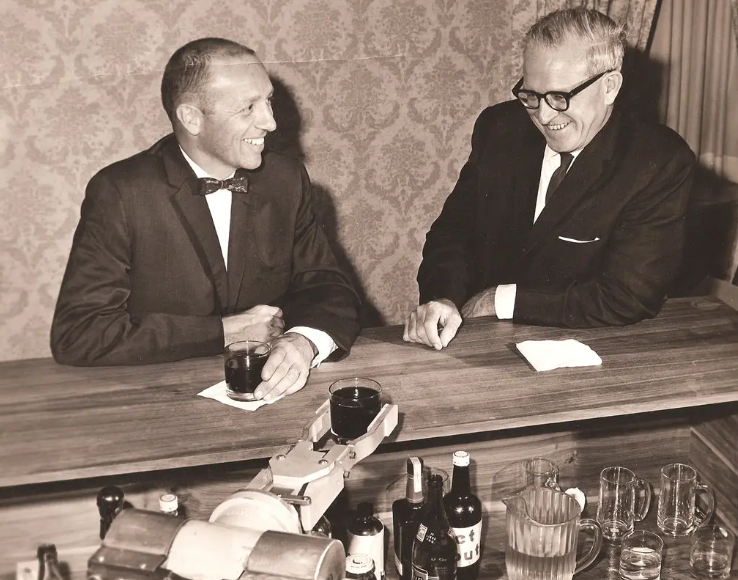
\includegraphics[width=62mm]{figs/Engelberger_Devol.png}}
      \hspace{2mm}
      \subfigure[Robot Unimate]{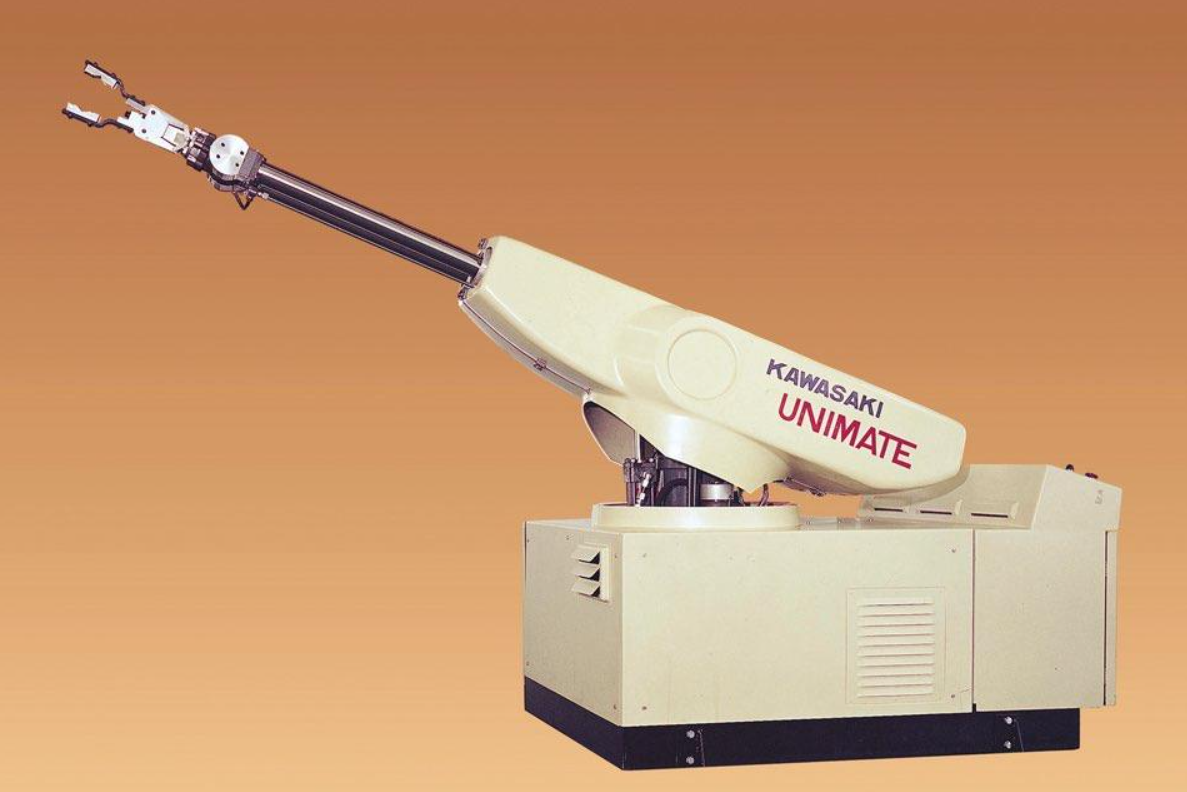
\includegraphics[width=73mm]{figs/Unimate robot.png}}
    \end{center}
    \caption{Primer robot industrial}
    \label{fig:primer_robot_industrial}
  \end{figure}
  
%Empresas como Ford y General Motors empezaron a plantearse la automatización de sus plantas productivas, por lo que, en 1962, la empresa AMF Corporation fabricó un nuevo robot llamado Versatan, un robot cilíndrico que Ford encargó para sus fábricas. Este robot, fue también el primero que se instaló en un centro productivo en Japón \cite{Gasparetto19}. \\

La segunda generación, o robots sensorizados (1968-1977), eran máquinas programables básicas con posibilidades limitadas de comportamiento autoadaptativo y capacidades elementales para reconocer el entorno externo, poseían sistemas sensoriales avanzados y eran robots de gran volumen que se utilizaban principalmente en automoción \cite{Zamalloa17}. \\

En 1968, en el Stanford Artificial Intelligence Laboratory (SAIL) se confecciona el WAVE, el primer lenguaje de programación para robots. En 1969, %Unimation concedió a Kawasaki Heavy Industries Ltd. la licencia para producir robots para el mercado japonés y asiático, conduciendo al desarrollo del Kawasaki-Unimate 2000, el primer robot industrial construido en Japón. Es también en este año cuando 
Víctor Scheinman, un estudiante de ingeniería mecánica de la Universidad de Standford, diseñó y construyó el primer prototipo de brazo robótico (Figura \ref{fig:standford_arm}), cuya cinemática inversa podía resolverse de manera analíticamente cerrada, permitiendo una rápida ejecución de la trayectoria \cite{Gasparetto19}. \\

  \begin{figure}[H]
    \begin{center}
      \subcapcentertrue
      \subfigure[Victor Scheinman con el Standford Arm]{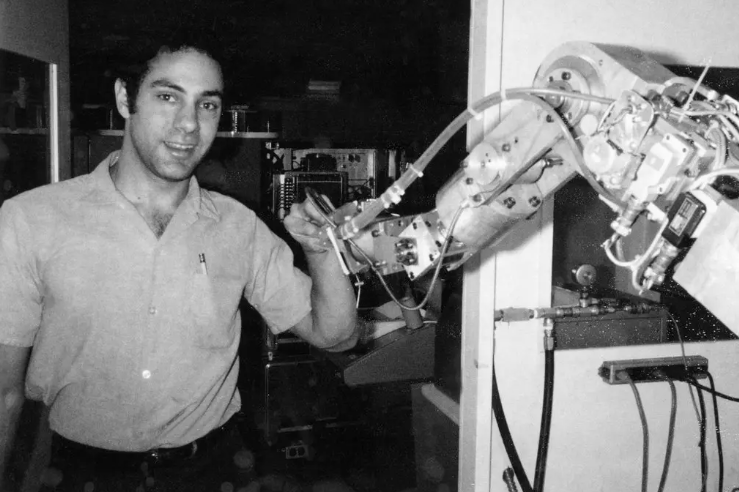
\includegraphics[width=62mm]{figs/Victor_Scheinman.png}}
      \hspace{2mm}
      \subfigure[Standford Arm]{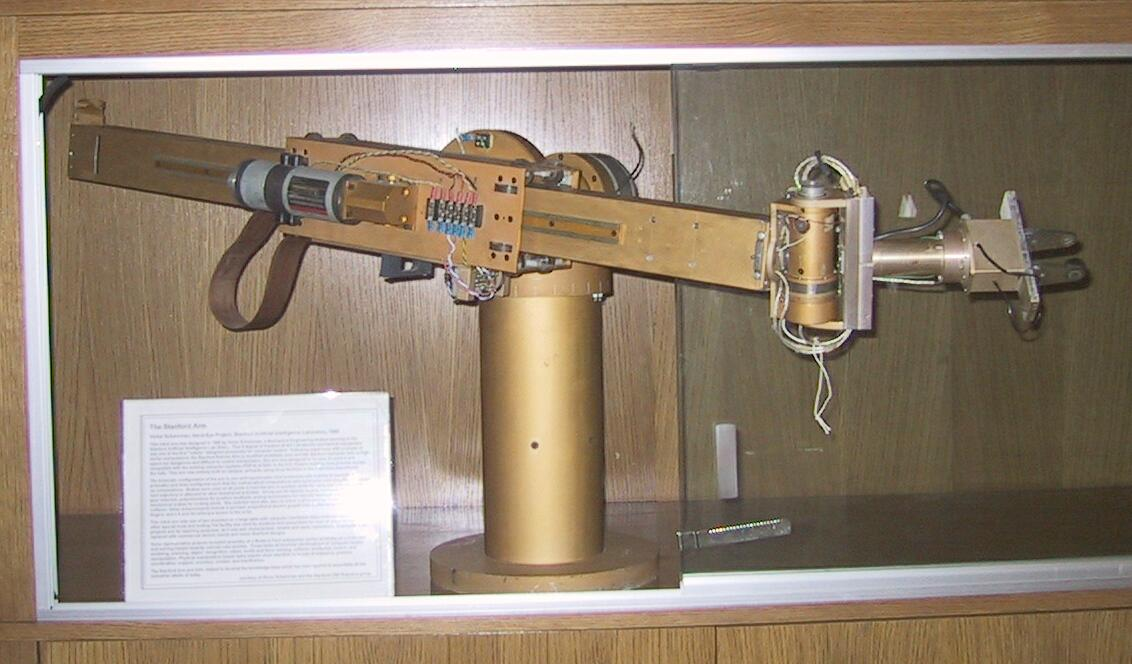
\includegraphics[width=71mm]{figs/Standford_arm.jpeg}}
    \end{center}
    \caption{Standford Arm}
    \label{fig:standford_arm}
  \end{figure}
 
%En 1969, el ingeniero de la compañía Yaskawa, T Mori, acuña el término mecatrónica, que integra el conjunto de mecanismos de control automático imprescindibles para el desarrollo de cualquier máquina inteligente \cite{Sanchez07b} tal y como muestra el diagrama de la Figura \ref{fig:Mecatrónica}.
  
  %\begin{figure} [h!]
   % \begin{center}
   %   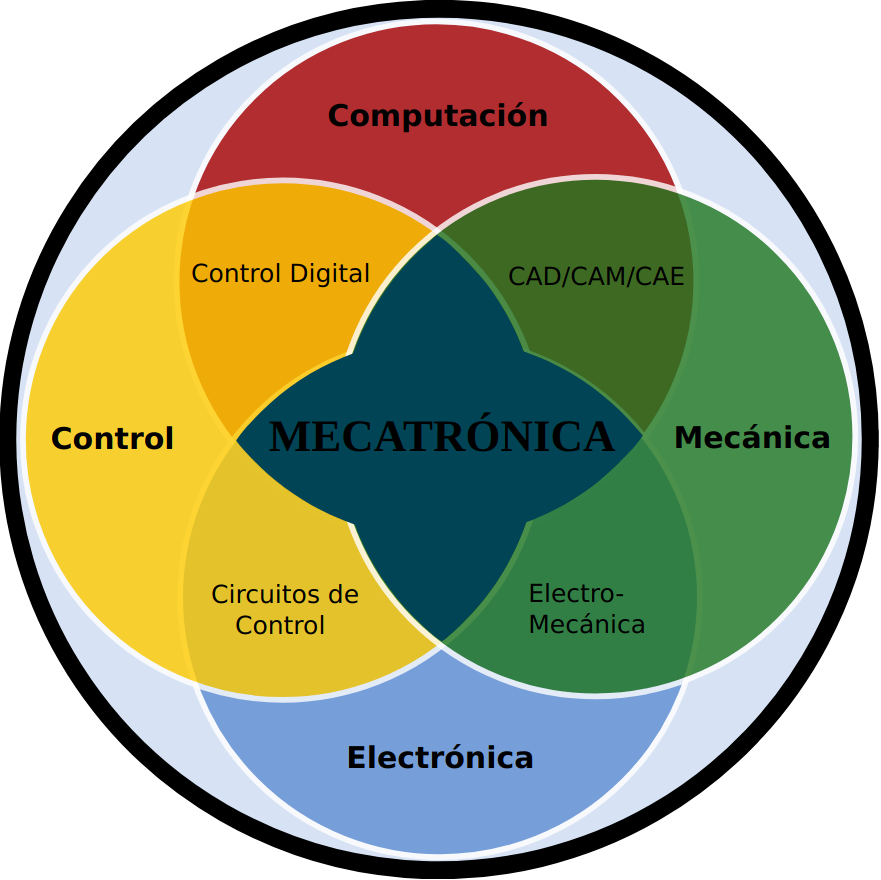
\includegraphics[width=65mm]{figs/meca.png}
   % \end{center}
   % \caption{Diagrama mecatrónico de construcción de máquinas inteligentes}
   % \label{fig:Mecatrónica}
  %\end{figure}
  
En 1973, KUKA\footnote{\url{https://www.kuka.com/es-es}} construyó el primer robot industrial con 6 ejes electromecánicos llamado Famulus. Un año más tarde, Cincinnati Milacron introdujo en el mercado el robot T3 (Figura \ref{fig:T3}). Cincinnati Milacron (adquirida por ABB\footnote{\url{https://new.abb.com/products/robotics}} en 1990). El robot T3 fue el primer robot comercial controlado por un microordenador \cite{Zamalloa17}.\\
  
  \begin{figure} [H]
    \begin{center}
      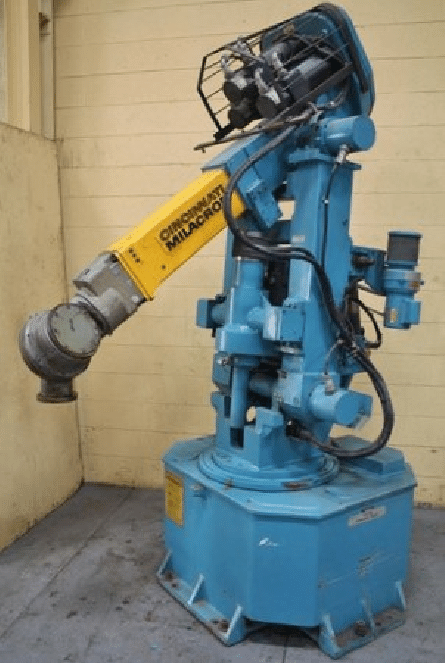
\includegraphics[width=55mm]{figs/T3_robot.png}
    \end{center}
    \caption{Robot Cincinnati Milacron T3}
    \label{fig:T3}
  \end{figure}
  
La tercera generación, o robots industriales (1978-1999), disponían de controladores específicos (ordenadores), siendo un punto clave en la caracterización de esta generación, además del surgimiento de nuevos lenguajes de programación para el control de los robots, la posibilidad de reprogramarlos y la inclusión parcial de la visión artificial \cite{Zamalloa17}.\\ %A finales de los años setenta y principios de los ochenta, otros avances científicos y técnicos contribuyeron a la difusión de los robots \cite{Gasparetto19}, que junto a que las empresas de todo el mundo invirtieron miles de millones de dólares en del mundo para automatizar tareas básicas en sus cadenas de montaje, supusieron que los robots poblaran muchos sectores industriales para automatizar una amplia variedad de actividades \cite{Zamalloa17}.\\ 
En 1978, Unimation diseñó y fabricó el robot PUMA. El PUMA (\textit{Programmable Universal Machine for Assembly}) fue considerado durante muchas décadas el arquetipo de los robots antropomórficos \cite{Gasparetto19}. Ese mismo año, el científico japonés Hiroshi Makino, de la Universidad de Yamanashi, propuso una nueva estructura cinemática. El robot con esta estructura se denominó SCARA (\textit{Selective Compliance Assembly Robot Arm})(ver Figura \ref{fig:Scara}), ya que su conformidad en la dirección horizontal resultó menor que la conformidad en la dirección vertical. Por esta razón, así como por la ligereza de la cadena cinemática (que permitía un controlador más sencillo y rápido), este robot era adecuado para ser empleado en tareas como el ensamblaje de objetos pequeños \cite{Makino80}.
  
  \begin{figure} [H]
    \begin{center}
      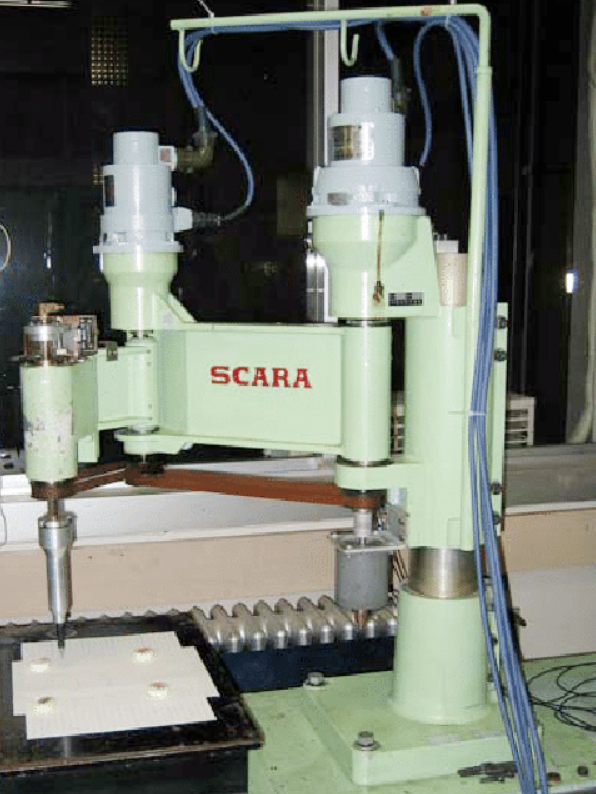
\includegraphics[width=45mm]{figs/Scara.png}
    \end{center}
    \caption{Uno de los primeros prototipos de robot SCARA}
    \label{fig:Scara}
  \end{figure}
  
%Más tarde, en 1981, en la Universidad Carnegie-Mellon se desarrolló un robot de impulsión directa que utiliza motores eléctricos en las articulaciones, evitando la distorsión de las transmisiones mecánicas convencionales. En 1982, IBM introduce el robot de montaje industrial RS-1 que utiliza un brazo constituido por 3 dispositivos de deslizamiento \cite{Sanchez07b}. De la idea de emplear cadenas cinemáticas paralelas en lugar de las clásicas cadenas cinemáticas en serie, junto con la de crear un robot ligero capaz de moverse a gran velocidad, surgió el arquetipo del robot Delta (que apareció en 1992), concebido por el científico suizo Reymond Clavel en la Escuela Politécnica Federal de Lausana (EPFL) \cite{Clavel91}. En comparación con los robots en serie, los robots paralelos tienen un espacio de trabajo más pequeño, pero pueden funcionar a una velocidad mucho mayor, siendo la arquitectura cinemática ideal para los robots dedicados a operaciones de pick-and-place de alta velocidad. 
Basado en este tipo de estructura, ABB desarrolló el Flex-Picker (Figura \ref{fig:Flexpicker_ABB}) en 1998, siendo este el robot de picking más rápido del mundo \cite{Gasparetto19}.\\
  
  \begin{figure} [H]
    \begin{center}
      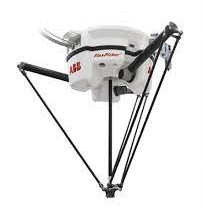
\includegraphics[width=45mm]{figs/flexpicker_ABB.jpeg}
    \end{center}
    \caption{Robot ABB IRB 360 Flexpicker}
    \label{fig:Flexpicker_ABB}
  \end{figure}
  
A partir del año 2000, aparece la cuarta generación o robots inteligentes (2000-Actualidad), que se caracteriza por la inclusión de capacidades informáticas avanzadas, ya que los ordenadores no sólo trabajan con datos, si no también pueden realizar razonamientos lógicos y aprender, puesto que la Inteligencia Artificial comienza a ser incluida parcial y experimentalmente en estos robots. Los sensores son más sofisticados, y envían información al controlador y la analizan mediante estrategias de control complejas para que el robot pueda basar sus acciones en información sólida y fiable. Es en esta generación cuando se introducen los robots colaborativos \cite{Zamalloa17}.\\
\pagebreak
  
Los requisitos de velocidad y peso de un robot han dado lugar a novedosos diseños cinemáticos y de transmisión. Desde el principio, la reducción de la masa y la inercia de las estructuras robóticas ha sido un objetivo primordial en el desarrollo de la robótica. El brazo humano, con una relación peso-carga de 1:1, se consideraba la referencia definitiva \cite{Siciliano16}. %Con este objetivo se desarrollaron, gracias a la colaboración entre la empresa alemana KUKA y el Instituto de Robótica y Mecatrónica del Centro Aeroespacial Alemán (DLR), tres generaciones de robots ligeros, permitiendo a investigadores e ingenieros desarrollar nuevas aplicaciones de robótica industrial y de servicios con un rendimiento sin precedentes. 
En el año 2004, con motivo de Automática, la mayor exposición de robots del mundo, se presentó por primera vez la combinación entre el robot ligero del DLR y la controladora KUKA, denominado RoboAssistant, donde se permitió a los visitantes mover y programar manualmente el robot, haciendo la visión de un robot que asiste a un trabajador durante los procesos de producción evidente para los visitantes \cite{Bischoff10}. \\
  
  
Es en estos procesos de producción, donde la manipulación a dos manos puede ser crítica para tareas de ensamblaje complejas, manipulación simultánea
y procesamiento de piezas de trabajo o para la manipulación de objetos de gran tamaño, por lo que en 2005, MOTOMAN presenta el primer robot comercial para la manipulación sincronizada a dos manos \cite{Siciliano16} (ver Figura \ref{fig:MOTOMAN}).\\

  \begin{figure} [H]
    \begin{center}
      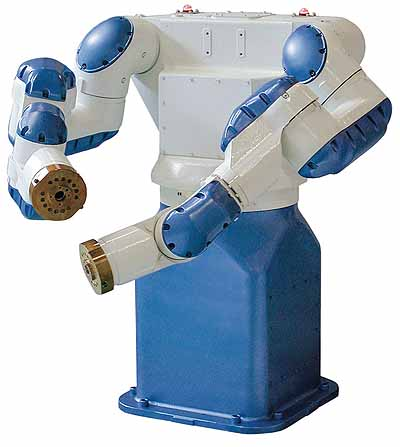
\includegraphics[width=55mm]{figs/MOTOMAN.jpg}
    \end{center}
    \caption{Robot Motoman DA-20}
    \label{fig:MOTOMAN}
  \end{figure}
  
Sin embargo, fue en el año 2006 %cuando, tras haber estado trabajando en la búsqueda de vías para el desarrollo en serie del robot LWR3 del DLR, y tras una intensa cooperación entre KUKA y el DLR para transmitir a los desarrolladores de KUKA los conocimientos necesarios para para el desarrollo de brazos ligeros, componentes y electrónica integrada, 
cuando se toma la decisión de producir una primera pequeña serie del robot ligero del KUKA LWR3 \cite{Bischoff10}, tal y como muestra la Figura \ref{fig:Lightweight Robot (LWR)}.
  
  \begin{figure}[H]
    \begin{center}
      \subcapcentertrue
      \subfigure[RoboAssistant en Automatica 2004]{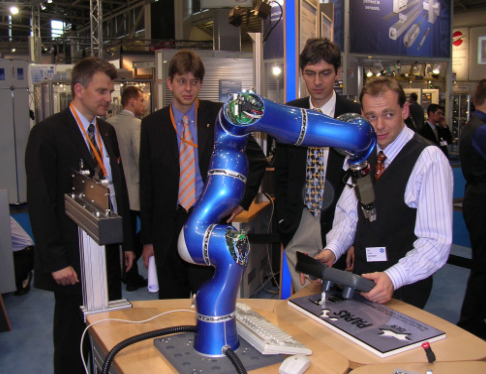
\includegraphics[width=72mm]{figs/RoboAssistant.png}}
      \hspace{2mm}
      \subfigure[Robot KUKA LWR3 con controladora (2006)]{\includegraphics[width=55mm]{figs/Kuka_lightweightrobot_2006.png}}
    \end{center}
    \caption{LWR3}
    \label{fig:Lightweight Robot (LWR)}
  \end{figure}
  
A principios de 2007, dos estudiantes de doctorado de la Universidad de Standford, Keenan Wyrobek y Eric Bergerlas, pusieron las primeras piezas de lo que eventualmente se convertiría en ROS (Robot Operating System). Uno de los preceptos principales que se tuvo en cuenta para la creación de este sistema operativo para robots fue el de crear un sistema que permitiese al máximo posible la reutilización de código, dando soporte a distintos tipos de robots y de aplicaciones. Esto resultó en la incorporación de ROS en una sorprendentemente amplia variedad de robots, extendiéndose incluso a dominios más allá de la comunidad académica de investigación a la que se dirigió inicialmente. Los años siguientes superaron todas las expectativas debido a que los avances en el ámbito de la robótica se compartieron de manera reproducible en ROS, y la Open Source Robotics Foundation (OSRF) se convirtió en el administrador principal de ROS en 2014. Con el objetivo de atender de manera más efectiva las demandas de una comunidad ROS más extensa y abordar sus nuevos escenarios de aplicación, la OSRF se dedicó a desarrollar ROS2 como un conjunto de paquetes paralelos que pudieran ser instalados junto a ROS1 (la versión original de ROS que nació en el año 2010, Figura \ref{fig:PR_ROS}) y ser compatibles entre sí. %Además, la popularidad de ROS ha seguido creciendo en la industria con el apoyo de proyectos como ROS-Industrial (ROS-I), una iniciativa de código abierto que extiende las capacidades avanzadas de ROS a hardware y aplicaciones industriales relevantes. \cite{Suarez22}.\\
  
  \begin{figure}[H]
    \begin{center}
      \subcapcentertrue
      \subfigure[Robot PR1]{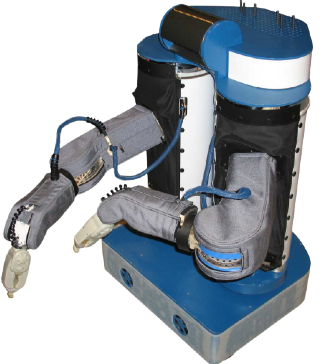
\includegraphics[width=52mm]{figs/PR1.png}}
      \hspace{2mm}
      \subfigure[Robot PR2]{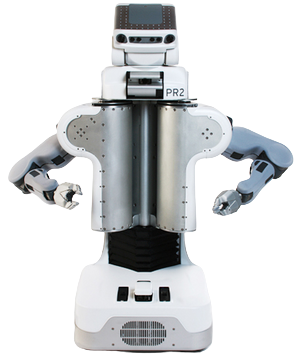
\includegraphics[width=50mm]{figs/PR2.png}}
    \end{center}
    \caption{Robots utilizados para el desarrollo de ROS}
    \label{fig:PR_ROS}
  \end{figure}
    
En el año 2008 se entrega el primer robot colaborativo o cobot, el UR5 de Universal Robots\footnote{\url{https://www.universal-robots.com/es/}} (Figura \ref{fig:UR5}), considerado como uno de los logros tecnológicos más significativos de la década en la comunidad robótica. El brazo robótico es pionero en la programación 3D fácil de usar pero sofisticada, con una interfaz de usuario intuitiva que permite a cualquier persona configurarlo y utilizarlo de forma rápida. Esta empresa, fundada en el año 2005 por Esteben Østergaard, Kasper Støy y Kristian Kassow tras conocerse en la Universidad de Dinamarca, surgió con el objetivo de hacer que la robótica sea accesible para las pequeñas y medianas empresas\footnote{\url{https://www.universal-robots.com/es/acerca-de-universal-robots/nuestra-historia/}}.\\
  
Esben H. Østergaard, Director de Tecnología y cofundador de Universal Robots, tomó el trabajo original de Peskhin y Colgate, dos investigadores de la empresa automovilística Ford de los años 90, que decidieron crear un nuevo robot industrial, más pequeño y ágil que los tradicionales, que saliera de su jaula para colaborar estrechamente con el ser humano en las tareas de calidad y personalización de los productos, sin embargo, no fueron capaces, puesto que el problema estaba en la relación entre seguridad y rendimiento, ya que el aumento de la primera reducía el de la segunda. Østergaard consiguió diseñar un sistema de seguridad y control para el cobot que lo bloquea en caso de colisión con el operario, %Como recuerda el propio Østergaard, la seguridad era la clave con la que la robótica colaborativa podía entrar en el escenario industrial. Así se creó un robot 
siendo capaz de operar en espacios confinados, en estrecho contacto con humanos, y sin instalar costosas barreras de seguridad \cite{Cusano22}.
  
  \begin{figure} [H]
    \begin{center}
      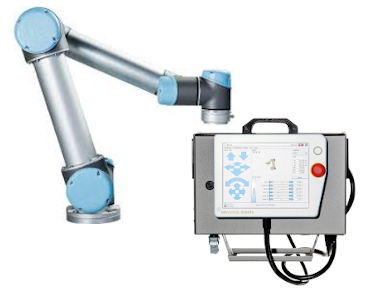
\includegraphics[width=75mm]{figs/UR5_controller.png}
    \end{center}
    \caption{UR5 con su controladora}
    \label{fig:UR5}
  \end{figure}
  
Más tarde, en 2018, Universal Robots presenta los robots colaborativos e-Series, que se pueden ver en la Figura \ref{fig:UR_e-Series}, que incluían avances tecnológicos que permitían un desarrollo más rápido para una mayor variedad de aplicaciones, ofrecía una programación más sencilla y seguía las normas de seguridad ISO más actuales y recientes\footnote{\url{https://www.universal-robots.com/es/acerca-de-universal-robots/nuestra-historia/}}.
 
  \begin{figure}[H]
    \begin{center}
      \subcapcentertrue
      \subfigure[UR presenta los  nuevos e-Series en Automatica 2018]{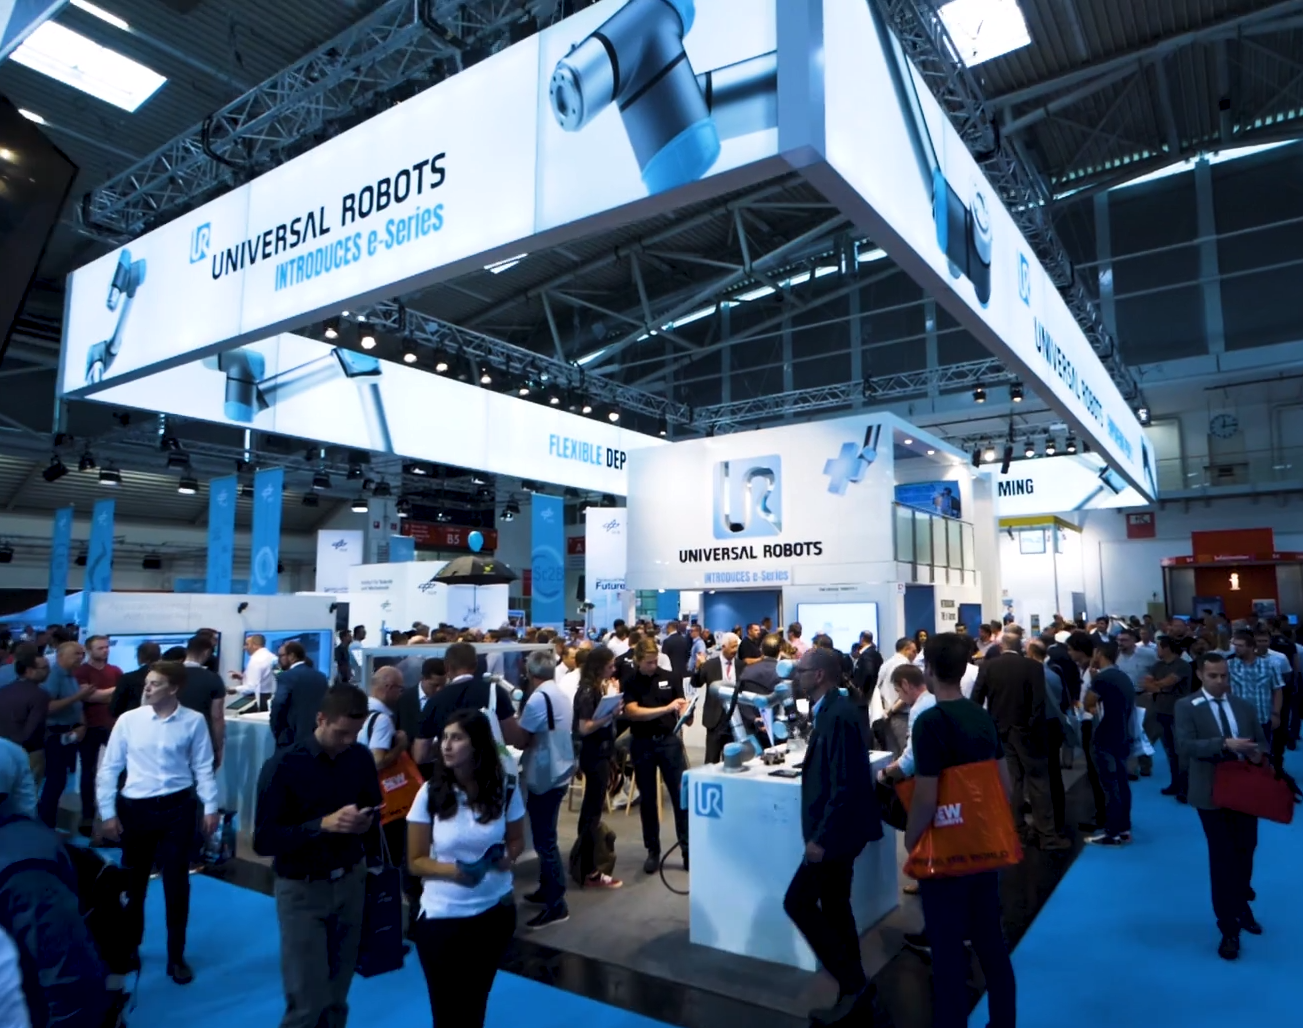
\includegraphics[width=75mm]{figs/UR Automatica 2018.png}}
      \hspace{2mm}
      \subfigure[UR e-Series]{\includegraphics[width=65mm]{figs/UR e-series.jpg}}
    \end{center}
    \caption{Universal Robots e-Series}
    \label{fig:UR_e-Series}
  \end{figure}

\pagebreak
Esta cuarta generación de robótica industrial ha establecido un sólido punto de partida para una continua revolución en el campo de la automatización. 
Es esencial destacar que varios de los modelos de robots mencionados previamente han seguido evolucionando y mejorando con el tiempo, siendo fruto de estas mejoras, la comercialización de nuevos modelos y series. 
Debido a que la tecnología se encuentra en constante desarrollo y a la colaboración cada vez más estrecha entre humanos y robots, el futuro de la robótica industrial promete seguir transformando radicalmente nuestros métodos de trabajo y producción, abriendo así nuevas oportunidades y desafiando constantemente los límites de lo que podemos lograr en la automatización industrial, así como en los otros dos grandes grupos de la robótica, como la robótica de servicio y la robótica médica.
   
\subsection{Robots de servicio}
\label{sec:robot_servicio}

Se define robot de servicio como un robot que realiza tareas útiles para las personas o los equipos, incluyendo en esta la manipulación o el servicio de artículos, el transporte, el apoyo físico, la orientación o información, el aseo personal, la cocina y la manipulación de alimentos y la limpieza en el ámbito personal; y la inspección, vigilancia, manipulación de objetos, transporte de personas, orientación o información, cocina y manipulación de alimentos y limpieza en el ámbito profesional \cite{ISO8373}.\\

%Su historia se remonta a la década de 1960, cuando surgieron los primeros intentos de crear robots para ayudar en tareas domésticas y de atención al cliente. Uno de los precursores de estos robots de servicio en 1968 fue el robot Shakey, desarrollado por el Laboratorio de Investigación de Inteligencia Artificial de Stanford (Stanford Research Institute, SRI). Shakey (ver en Figura \ref{fig:shakey}), provisto de múltiples sensores y medios para desplazarse por el suelo, además de control remoto por radio \cite{Sanchez07b}, podía realizar tareas de planificación, búsqueda de rutas y reordenación de objetos sencillos, siendo el primer robot móvil con capacidad para percibir y razonar sobre su entorno\footnote{\url{https://www.sri.com/hoi/shakey-the-robot/}}. 

%  \begin{figure} [H]
%    \begin{center}
%      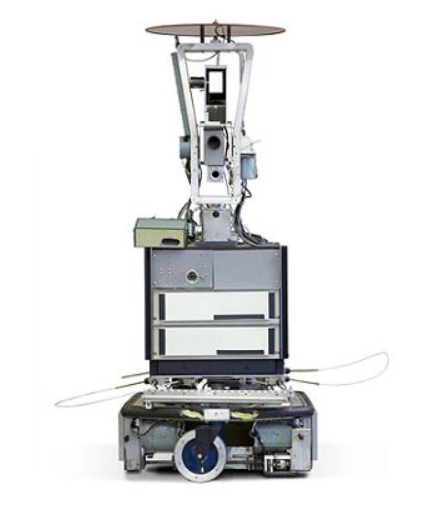
\includegraphics[width=65mm]{figs/Shakey.png}
%    \end{center}
%    \caption{Robot Shakey}
%    \label{fig:shakey}
%  \end{figure}
     
%Sin embargo, fue a mediados de los años 80 cuando en los laboratorios y centros de investigación dedicados a la robótica se trató de revitalizar la importancia de los robots en nuestra sociedad, planteando las ventajas que el uso del robot podía traer en tareas en las que el ser humano asumía riesgos o en las que las capacidades de aquel estaban limitadas por factores como la fuerza o la precisión necesaria. Fue precisamente al entenderse que estas nuevas aplicaciones de la robótica no tenían un uso industrial con el objetivo de fabricar bienes, sino que se trataba de un empleo para desarrollar tareas para las personas, cuando se catalogaron como aplicaciones en el sector servicios \cite{Barrientos02}(ver ejemplos en la Figura \ref{fig:Robots_servicio}).\\

En la práctica, las actuales y potenciales aplicaciones no industriales de los robots son tan variadas y diferentes que se dificulta su catalogación \cite{Barrientos02}; sin embargo, existen ciertas características especiales en estos robots de servicio %(ver ejemplos en la Figura \ref{fig:Robots_servicio})
que los hacen diferentes de los robots industriales \cite{Aracil08}, y los caracterizan para llevar a cabo estas tareas para las personas, siendo las principales características estos tres atributos de diseño: representación, antropomorfismo y orientación a la tarea, es decir, los robots de servicio pueden tener una representación física %(por ejemplo, Pepper) 
o tener una representación únicamente virtual %(por ejemplo, Alexa, ya que el software de IA virtual que funciona de forma autónoma y aprende con el tiempo también puede clasificarse como robot de servicio)
, diseñarse como humanoides (es decir, antropomorfos) simulando una apariencia humana o como no humanoides %(por ejemplo, el robot de limpieza Roomba de iRobot \footnote{\url{https://www.irobot.es/}} (Figura \ref{fig:roomba})
, y pueden realizar tareas analíticas %gracias a la potencia informática subyacente 
o tareas emocionales-sociales (por ejemplo, robots de recepción) \cite{Wirtz18}.\\

% \begin{figure}[H]
%    \begin{center}
%      \subcapcentertrue
%      \subfigure[Alexa]{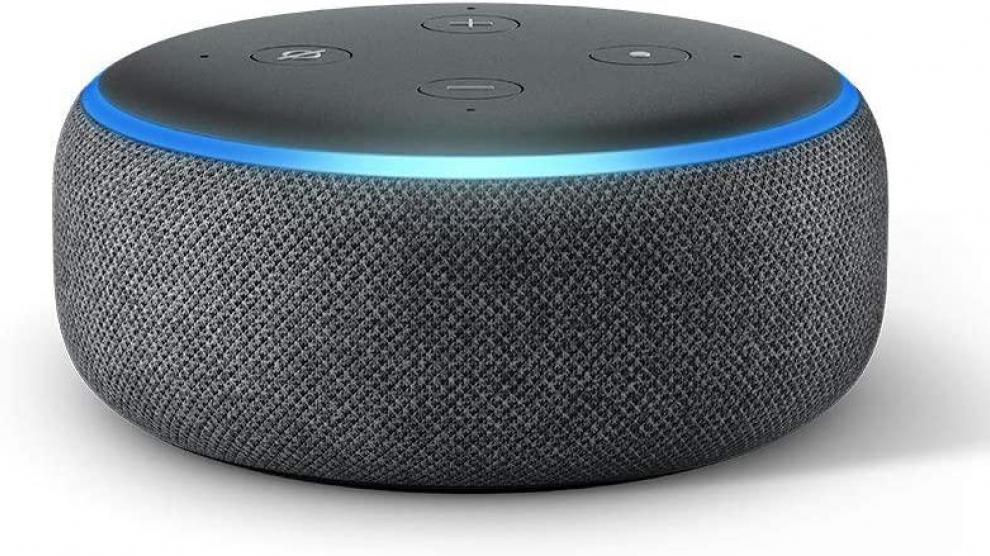
\includegraphics[width=45mm]{figs/Alexa.jpeg}}
%      \hspace{2mm}
%      \subfigure[Pepper]{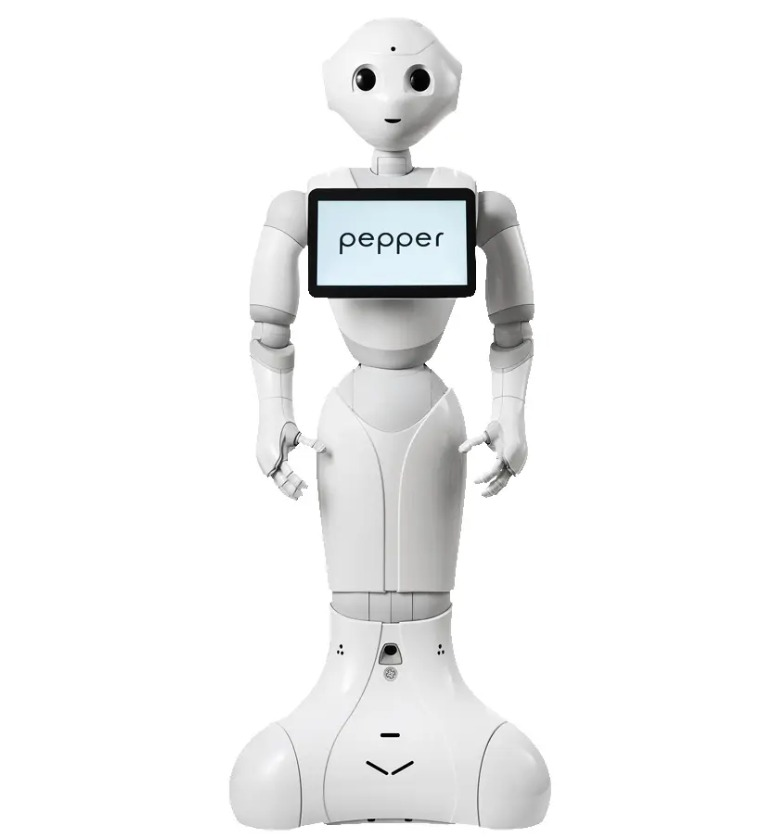
\includegraphics[width=45mm]{figs/Pepper.jpeg}}
%      \hspace{2mm}
%      \subfigure[Sophia]{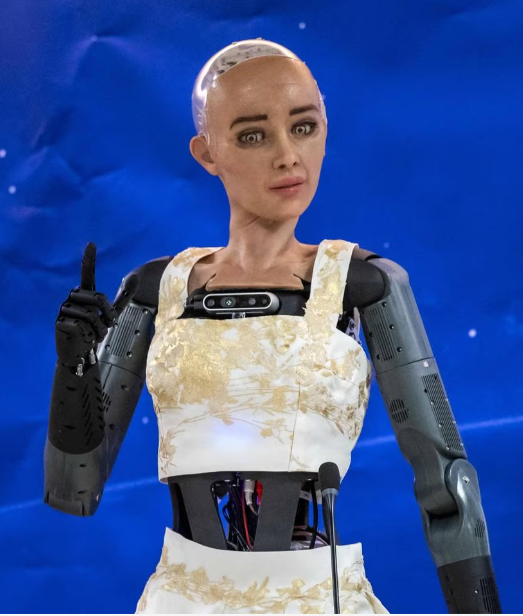
\includegraphics[width=38mm]{figs/Sophia.png}}
%    \end{center}
%    \caption{Robots de servicio}
%    \label{fig:Robots_servicio}
%  \end{figure}

Tratando de establecer una división de los robots de servicio, la norma ISO 8373:2012, así como la Federación Internacional de Robótica o IFR, propuso clasificarles en diferentes categorías según su función y aplicación en robots para uso doméstico y personal y robots de servicio destinados a un uso profesional \cite{Gonzalez21}, siendo las aplicaciones más importantes las siguientes:

\begin{itemize}
 \item \textit{Limpieza:} Suelen estar equipados con sensores y tecnología de navegación que les permite moverse de manera autónoma por el espacio, detectar obstáculos y llevar a cabo actividades de limpieza de manera eficiente. 
 
 \begin{figure} [H]
  \begin{center}
    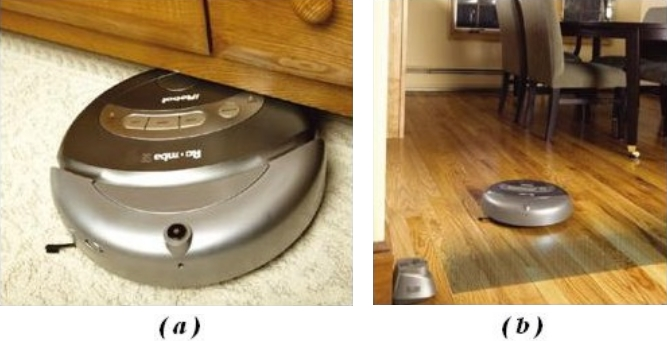
\includegraphics[width=90mm]{figs/roomba}
  \end{center}
  \caption{Robot aspirador Roomba de iRobot}
  \label{fig:roomba}
 \end{figure}
 
 \item \textit{Inspección y mantenimiento:} Son máquinas diseñadas para llevar a cabo tareas de supervisión, evaluación y mantenimiento en entornos de infraestructura o áreas de difícil acceso. Estos robots suele ser máquinas autónomas o teleoperadas equipadas con sensores, cámaras y herramientas especializadas que les permiten evaluar, reparar y mantener equipos, estructuras y sistemas en entornos desafiantes o peligrosos. 
 
 \begin{figure}[H]
    \begin{center}
      \subcapcentertrue
      \subfigure[Spot de Boston Dynamics]{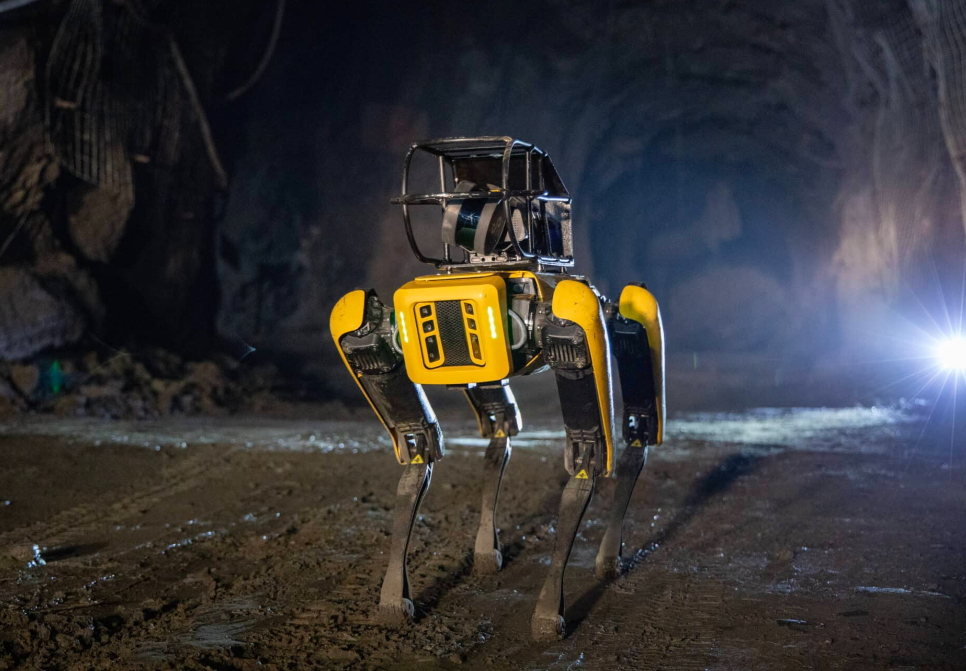
\includegraphics[width=60mm]{figs/Spot.png}}
      \hspace{2mm}
      \subfigure[ROBTET, robot para el mantenimiento de líneas de alta tensión]{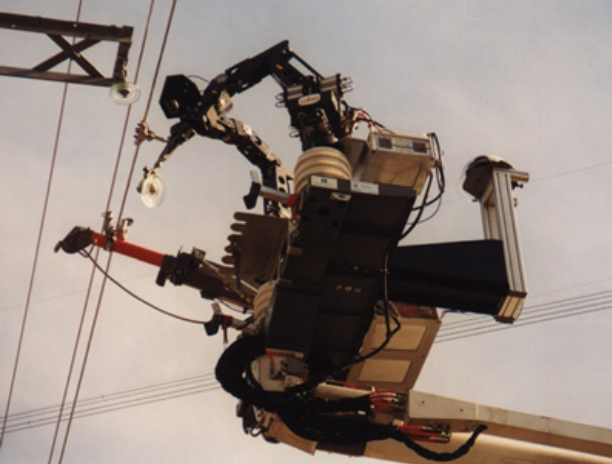
\includegraphics[width=55mm]{figs/ROBTET.png}}
    \end{center}
    \caption{Robots de inspección y mantenimiento}
    \label{fig:Robots de inspección y mantenimiento}
  \end{figure}
 
 
 \item \textit{Educación:} %Aquellos robots utilizados en educación 
Son robots diseñados para facilitar el aprendizaje y la enseñanza en los diferentes niveles educativos%. Estos robots 
, pudiendo ser utilizados en aulas, bibliotecas y entornos de aprendizaje para ayudar a los estudiantes a adquirir habilidades, fomentar la creatividad y brindar experiencias educativas interactivas.\\
 
 \begin{figure}[H]
    \begin{center}
      \subcapcentertrue
      \subfigure[Robot NAO]{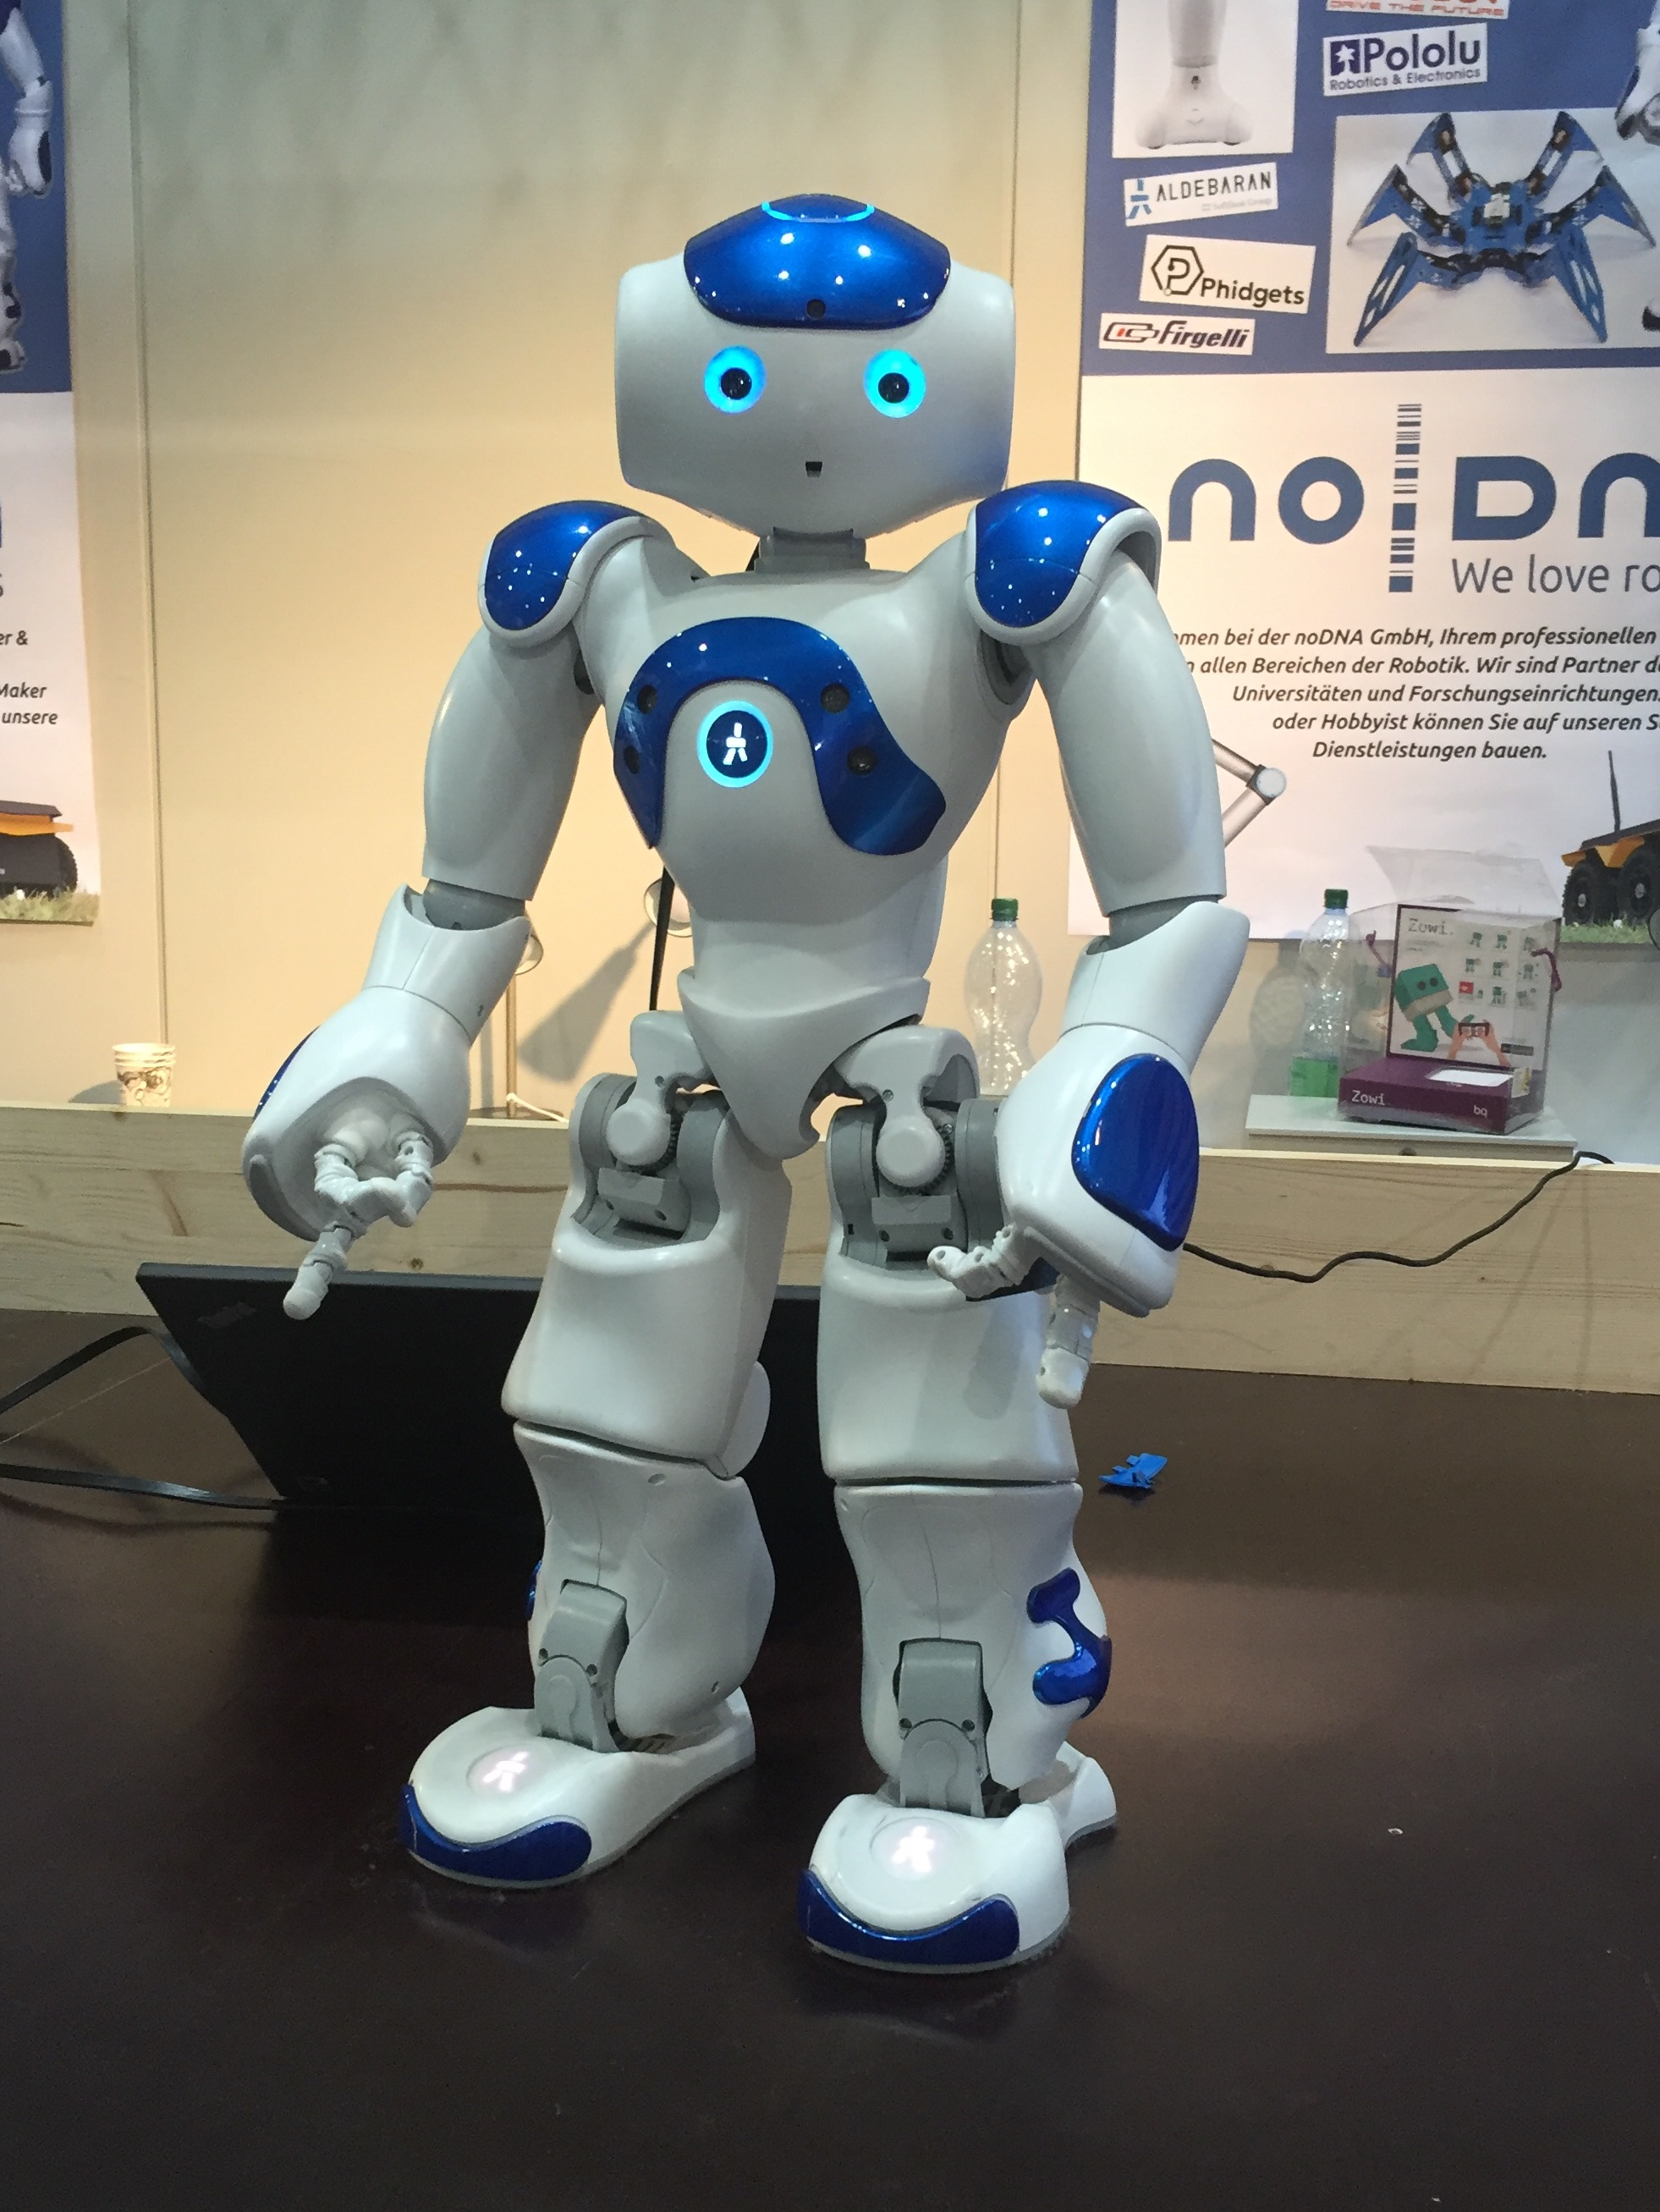
\includegraphics[width=40mm]{figs/Robot NAO.jpg}}
      \hspace{2mm}
      \subfigure[Turtlebot 4]{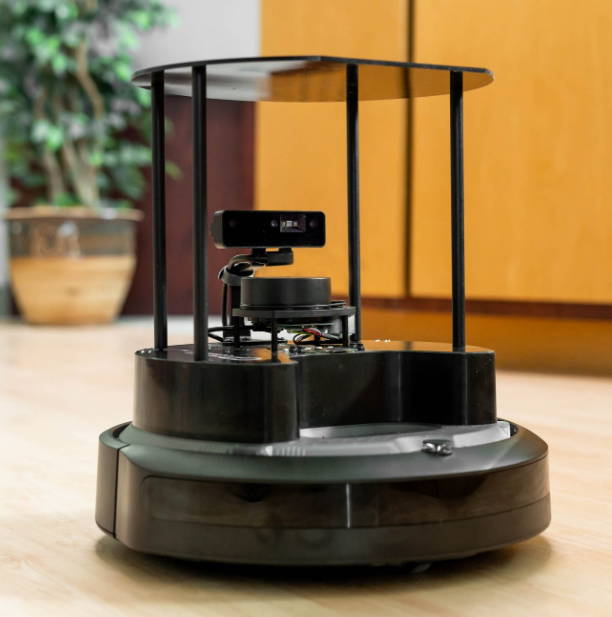
\includegraphics[width=53mm]{figs/Turtlebot 4.png}}
    \end{center}
    \caption{Robots de educación}
    \label{fig:Robots de educación}
  \end{figure}
 
 \item \textit{Logística:} Los robots de servicio utilizados en logística son robots diseñados para llevar a cabo tareas relacionadas con la gestión y el movimiento de mercancías y productos en entornos de almacenamiento, distribución y transporte. Estos robots desempeñan un papel fundamental en la optimización de la cadena de suministro, mejorando la eficiencia y la precisión en la manipulación de productos. Un ejemplo del posible uso de estos robots en el sector agrícola, es la primera granja vertical de interior del mundo en Estados Unidos, que producirá 18 millones de kilogramos de fresas al año, marcando un hito en la agricultura moderna, y demostrando que la automatización e integración de la robótica en este tipo de granjas verticales puede transformar la producción y recolección de alimentos a gran escala \cite{EcoInventos24}.
 
% \begin{figure} [H]
%  \begin{center}
%    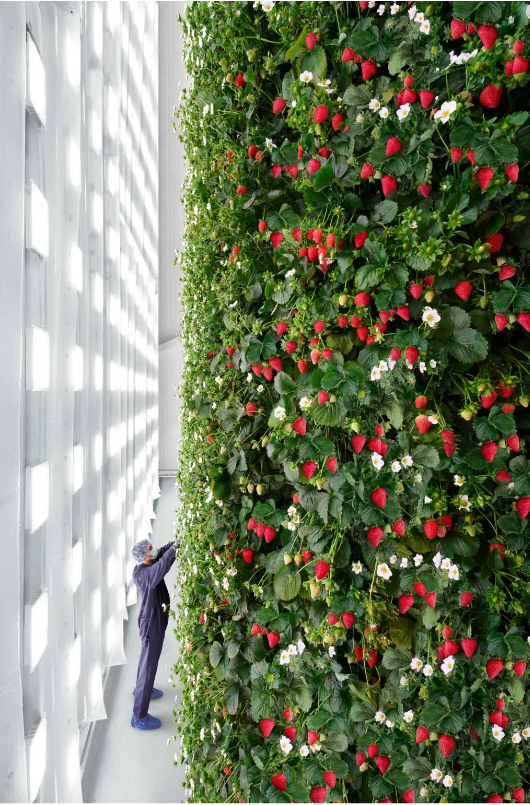
\includegraphics[width=50mm]{figs/agricultura vertical 1.png}
%  \end{center}
%  \caption{Agricultura vertical}
%  \label{fig:agricultura_vertical}
% \end{figure}
 
%Por otro lado, dentro de los robots de logística empleados para el movimiento de mercancías, se pueden distinguir dos grandes grupos: Vehículos Guiados Automáticos (AGV) y Robots Móviles Autónomos (AMR). La principal diferencia entre los AMR y los AGV radica en la capacidad de adaptación y autonomía, ya que los AMR son altamente flexibles, autónomos y versátiles, con capacidades autónomas avanzadas que les permiten ajustarse rápidamente a cambios en los entornos de trabajo, mientras que los AGV siguen rutas predefinidas y son adecuados para tareas de transporte predecibles en entornos más controlados.
 
 \begin{figure}[H]
    \begin{center}
      \subcapcentertrue
      \subfigure[AGV Robots Kiva de Amazon]{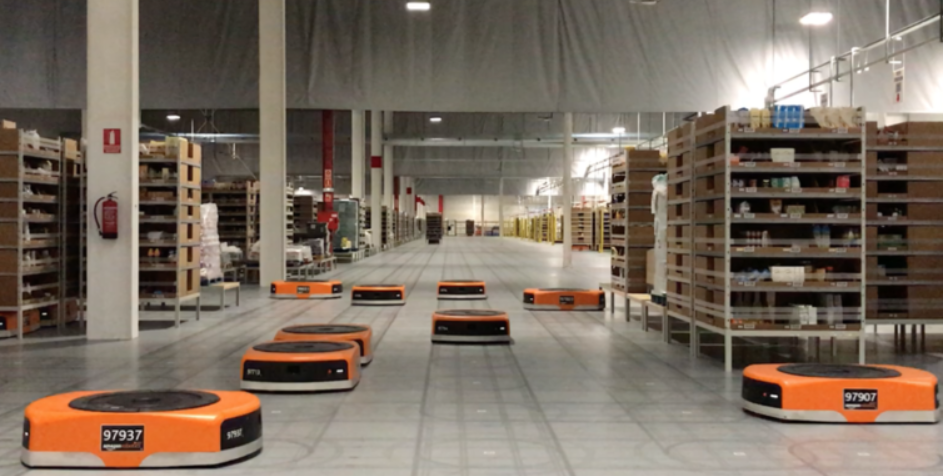
\includegraphics[width=67mm]{figs/AGV Amazon.png}}
      \hspace{2mm}
      \subfigure[AMRs de MiR]{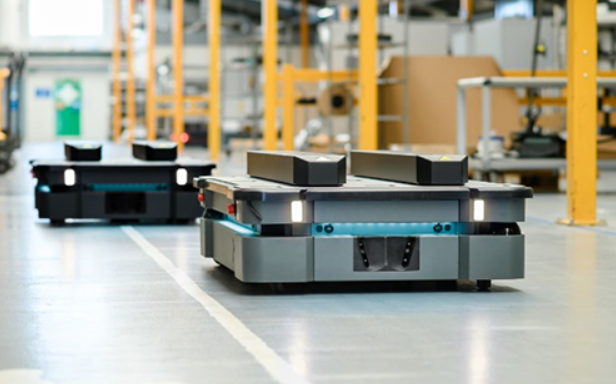
\includegraphics[width=55mm]{figs/MiR.png}}
    \end{center}
    \caption{Robots de logística}
    \label{fig:Robots de logística}
  \end{figure}
  
 \pagebreak 
 \item \textit{Entretenimiento:} Son robots diseñados específicamente para proporcionar experiencias lúdicas y de entretenimiento a las personas. Estos robots se utilizan en una variedad de contextos, siendo máquinas robóticas diseñadas para interactuar con el público. 
 
  \begin{figure}[H]
    \begin{center}
      \subcapcentertrue
      \subfigure[SONY Aibo]{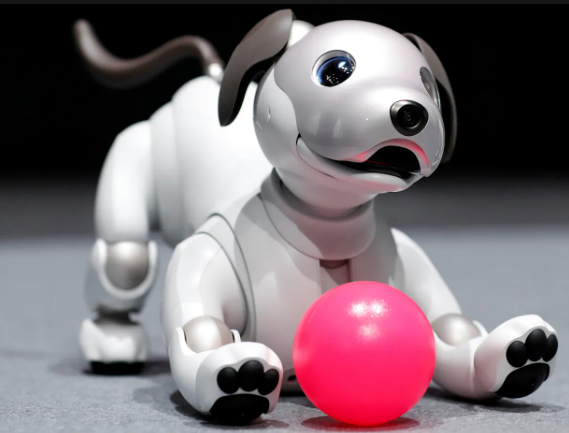
\includegraphics[width=50mm]{figs/SONY Aibo.png}}
      \hspace{2mm}
      \subfigure[Dron DJI Spark]{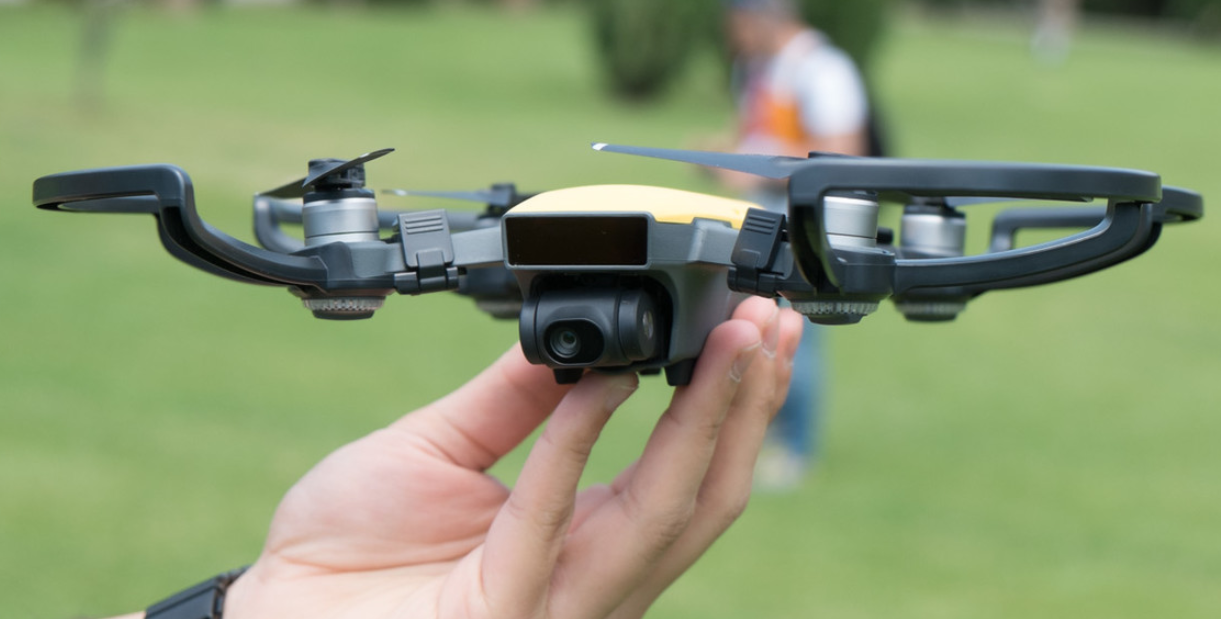
\includegraphics[width=76mm]{figs/Dron DJI Spark.png}}
    \end{center}
    \caption{Robots de entretenimiento}
    \label{fig:Robots_entretenimiento}
  \end{figure}
   
\end{itemize}

La robótica de servicio representa una revolución en la asistencia y el apoyo a diversas industrias, desde la logística hasta la atención al cliente en el comercio minorista. Sin embargo, su impacto va más allá, extendiéndose hasta la atención médica. En este contexto, la robótica médica emerge como una vanguardia tecnológica que fusiona la innovación robótica con la medicina moderna para ofrecer soluciones innovadoras en diagnóstico, tratamiento y rehabilitación, demostrando su potencial para revolucionar la forma en que brindamos y recibimos atención médica.
 
\subsection{Robots médicos}
\label{sec:robotica_industrial} 

Se define \textit{robot médico} como aquellos dispositivos electromecánicos que desempeñan parcial o totalmente algunas funciones de los seres humanos o de sus órganos al resolver problemas médicos, ayudando a mejorar la asistencia al paciente y los resultados, a la vez que aumenta la eficiencia operativa \cite{Kraevsky10}.\\

Los robots médicos se desarrollaron por primera vez hace poco más de tres décadas para permitir a los cirujanos operar a sus pacientes a distancia o con mayor precisión. A finales de los años noventa, había 2 tipos de telemanipuladores quirúrgicos aprobados por la Administración de Alimentos y Medicamentos de los Estados Unidos (FDA): el Zeus y el da Vinci (Figura \ref{fig:RobotDaVinci}), introducido en 1998-1999, que permitía aumentar la precisión de las cirugías mínimamente invasivas (CMI) \cite{Romero20}.\\

\begin{figure} [H]
    \begin{center}
      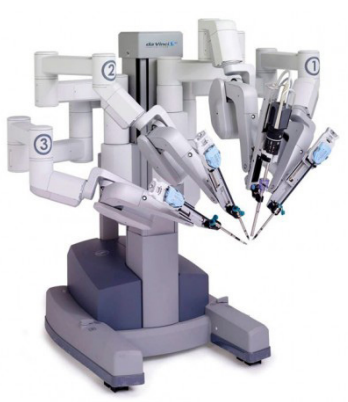
\includegraphics[width=10cm]{figs/Robot Da Vinci.png}
    \end{center}
    \caption{Robot Da Vinci}
    \label{fig:RobotDaVinci}
\end{figure}

Las primeras aplicaciones fueron en los campos de neurocirugía y cirugía ortopédica, siendo la cirugía donde mayor impacto han tenido los robots médicos, %A medida que se ha hecho patente la aceptación de los robots quirúrgicos por nuestros sistemas sanitarios, los investigadores en robótica han ido centrando cada vez más su atención en cómo podría ser la próxima generación de robots médicos. Su atención no se limita a los robots quirúrgicos, y también 
sin embargo, se están investigando otras áreas de la medicina, como los robots para realizar rehabilitación física con pacientes con discapacidades motores, como el exoesqueleto Ekso Bionics, robots de telepresencia para la interacción del paciente con el personal sanitario externo, como el robot RP-VITA, automatización de farmacias, robots para desinfectar clínicas, etc. \cite{Dupont21}\\

% \begin{figure}[H]
%    \begin{center}
%      \subcapcentertrue
%      \subfigure[Exoesqueleto Ekso Bionics]{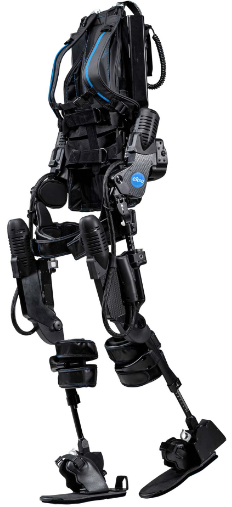
\includegraphics[width=35mm]{figs/Ekso Bionics.png}}
%      \hspace{20mm}
%      \subfigure[Robot RP-VITA]{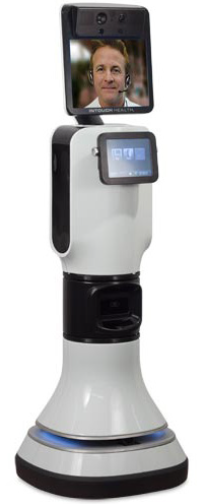
\includegraphics[width=35mm]{figs/RP Vita.png}}
%    \end{center}
%    \caption{Robots médicos}
%    \label{fig:Robots_medicos}
%  \end{figure}

El rápido crecimiento de la robótica médica se debe a una combinación de mejoras tecnológicas (motores, materiales y teoría de control), los avances en imagen médica (mayor resolución, resonancia magnética y ecografía 3D) y una mayor aceptación por cirujanos y pacientes de los procedimientos laparoscópicos y la asistencia robótica \cite{Beasley12}, convirtiéndose en un campo interdisciplinario que abarca desde cirugía asistida por robots hasta sistemas de diagnóstico de vanguardia. Gran parte de su éxito radica en la integración de tecnologías avanzadas, como la inteligencia y la visión artificial. Estas disciplinas están redefiniendo la forma en que los robots médicos pueden interactuar con el entorno, interpretar datos y, en última instancia, mejorar los resultados en la atención médica.\\

A continuación, explicaremos el impacto que la inteligencia y la visión artificial están teniendo en la robótica, y las capacidades y oportunidades que estas presentan en una inmensa variedad de aplicaciones.

\section{Inteligencia Artificial}
\label{sec:IA} 

La Inteligencia Artificial (IA) es un área multidisciplinaria de la ciencia %de gran interés por ser un área multidisciplinaria 
donde se realizan sistemas que tratan de hacer tareas y resolver problemas como lo hace un humano;así mismo, trata de simular de manera artificial las formas de pensamiento y de trabajar del cerebro para la toma de decisiones \cite{Ponce14}.\\

El origen del concepto y de los criterios de desarrollo de la IA se remontan al año 1936, con el matemático inglés Alan Turing, quien definió una máquina abstracta como ya vimos en la sección \ref{sec:robótica}, que sirvió de base de la noción de algoritmo y la definición de clase de problemas deducibles \cite{Hardy01}, y quien intuyó la importancia que jugaría el aprendizaje automático en el desarrollo de la IA al afirmar que, en lugar de intentar emular mediante una máquina la mente de un adulto, quizá sería más factible intentar emular la mente de un niño y luego someter a la máquina a un proceso de aprendizaje que diera lugar a un desarrollo cognitivo de dicha mente hasta alcanzar el equivalente de una mente adulta, lo que actualmente se conoce como robótica de desarrollo \cite{Gonzalez17}, mientras que el apelativo Inteligencia Artificial se debe a John McCarthy, quien organizó una conferencia en el Darmouth College (Estados Unidos) en agosto de 1956, para discutir sobre la posibilidad de construir máquinas inteligentes. Como resultado de esta reunión, se establecieron los primeras bases sobre la inteligencia de los computadores \cite{Ponce14}.\\ 

%La historia de la IA ha sido testigo de ciclos caracterizados por la introducción de nuevos y creativos enfoques y de un sistemático perfeccionamiento de los mejores. Estos ciclos de avance y desafío continúan moldeando su evolución y prometen un futuro emocionante y lleno de posibilidades.\\

Dentro de las diversas formas de clasificar la IA, existe una clasificación, como se muestra en la Figura \ref{fig:ModelosInteligencia}, que se basa en el objetivo y la forma en que trabaja el sistema: sistemas que piensan como humanos, sistemas que actúan como humanos, sistemas que piensan racionalmente, y sistemas actuantes racionales. Esta clasificación de manera inicial se veía como clases independientes, sin embargo, en la actualidad los sistemas mezclan características de ellas. \cite{Ponce14} \\

\begin{figure} [H]
    \begin{center}
      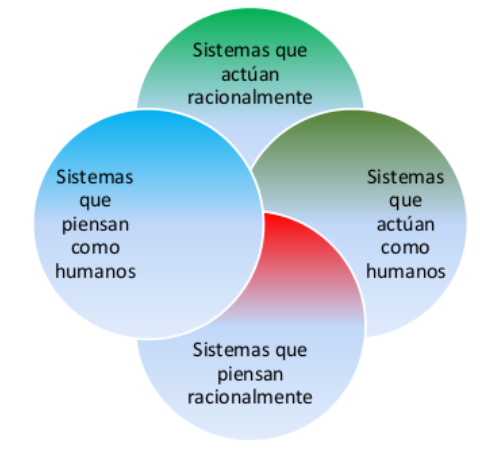
\includegraphics[width=9cm]{figs/Modelos de inteligencia.png}
    \end{center}
    \caption{Modelos de inteligencia}
    \label{fig:ModelosInteligencia}
\end{figure}

%La clasificación de los modelos de IA tiene un impacto significativo en las aplicaciones de la IA, ya que determina cómo se desarrollan y aplican los sistemas de inteligencia artificial en una amplia gama de campos, contribuyendo así a la mejora de la eficiencia y la innovación en muchas industrias donde se han ido desarrollando diferentes herramientas propias y aplicaciones, dando lugar a multitud de ramas que parten de la IA.\\

Una de las ramas más fascinantes y prometedoras de la inteligencia artificial es la visión artificial, que busca dotar a las máquinas de la capacidad de interpretar y comprender el mundo visual que les rodea. La siguiente sección se centra en la importancia de la IA y su intersección con la visión artificial, explorando cómo estas disciplinas se fusionan para mejorar la percepción y la comprensión de imágenes y vídeos.

\section{Visión Artificial}
\label{sec:VA} 

La visión artificial se define como la ciencia de programar un ordenador para procesar imágenes o vídeos e incluso entenderlos \cite{Culjak12}.\\

En \cite{Bradski08} se explica cómo es la transformación de datos desde un fotograma o vídeo cámara hasta lo que puede ser una decisión o una nueva representación \cite{Alvear17}. Para ello, la imagen percibida pasa por los procesos de obtención, caracterización e interpretación de información de imágenes; y estos procesos pueden ser subdivididos a su vez en \cite{Santillan15} según el Cuadro \ref{cuadro:procesos_VA}.\\

\begin{table} [H]
  \begin{center}
      \includegraphics[width=15cm, height=7cm]{figs/Procesos de la visión artificial.png}
  \end{center}
  \caption{Procesos de la visión artificial}
  \label{cuadro:procesos_VA}
\end{table}

\begin{enumerate}
 \item \textit{Captura:} %La captura o digitalización 
Es el proceso en el que se obtiene una imagen digital a partir de una imagen analógica a través de un dispositivo para que pueda ser manipulada por un ordenador. Esta imagen estará representada como una matriz de números (píxeles) \cite{Martinez22}.
 
 \item \textit{Pre-procesamiento:} En esta fase, se incorporan métodos destinados a restaurar las imágenes capturadas.%, dado que es factible que las imágenes experimenten deterioro.%, como la disminución de su claridad o la presencia de ruido. 
Esta etapa tiene como objetivo corregir estos problemas mediante procedimientos como la eliminación de ruido o la mejora del contraste y la nitidez.
 
 \item \textit{Segmentación:} %La segmentación 
Consiste en dividir una imagen en regiones o componentes más pequeños (grupo de píxeles) con el objetivo de identificar y aislar objetos o áreas de interés dentro de la imagen %El propósito principal es simplificar y organizar la información visual contenida en la imagen 
para que sea más fácil de analizar, comprender y procesar por ordenador.

 \item \textit{Descripción:} Es el proceso que obtiene características relevantes para poder diferenciar un tipo de objeto de otro, pudiendo ser externas, como la forma, el perímetro o el rectángulo mínimo que contiene la región; o internas, como el área o el centro de gravedad, entre otros \cite{Santillan15}. 
 
 \item \textit{Reconocimiento (clasificación):} %Esta fase se centra en identificar y asignar etiquetas o categorías a objetos o patrones previamente segmentados en una imagen o secuencia de imágenes. 
El proceso de reconocimiento implica el uso de algoritmos y técnicas de aprendizaje automático, como redes neuronales artificiales o métodos estadísticos, entre otros, para entrenar un modelo que pueda tomar las características extraídas y realizar predicciones sobre la clase o categoría a la que pertenecen los objetos detectados.
 
 \item \textit{Interpretación:} %Esta fase implica el análisis y comprensión del significado y el contexto de la información visual obtenida de las imágenes o la secuencia de imágenes capturadas. 
Esta etapa implica razonamiento, toma de decisiones y puede requerir el procesamiento de lenguaje natural para obtener una comprensión más profunda del contenido visual.
 
\end{enumerate}

Estas fases son las empleadas bajo el paradigma de lo que se conoce como Visión
Artificial Clásica, enfocada a la utilización de algoritmos específicos para procesar imágenes y reconocer en ellas características básicas \cite{Martinez22}.%, siendo generalmente secuenciales, a pesar de que los procesos que se utilicen en la resolución de un determinado problema dependen de su complejidad y no todas pueden ser siempre necesarias \cite{Santillan15}.\\
Sin embargo, para mejorar aún más la eficacia de los sistemas de visión artificial, se recurre al aprendizaje automático o \textit{machine learning} (ML). A continuación, profundizaremos en el papel del \textit{machine learning} en la visión artificial y su importancia en la creación de sistemas inteligentes de procesamiento de imágenes. 

\section{Machine Learning}
\label{sec:MachineLearning} 

El Machine Learning (Aprendizaje Automático) es una rama en evolución de la Inteligencia Artificial que se encarga de generar algoritmos que tienen la capacidad de aprender del entorno circundante y no tener que programarlos de manera explícita, teniendo en cuenta todos los escenarios posibles, a partir de la construcción de modelos analíticos \cite{Sandoval18}.\\ %Los aspectos clave y la semántica del machine learning se muestran en la Figura \ref{fig:ML semantics}.

% \begin{figure} [H]
%    \begin{center}
%      \includegraphics[width=14cm]{figs/ML semantics.png}
%    \end{center}
%    \caption{Aspectos clave y semántica del Aprendizaje automático}
%    \label{fig:ML semantics}
% \end{figure}

%En función del problema planteado y de los datos disponibles, se pueden distinguir tres tipos de ML:

%\begin{itemize}
% \item \textit{Aprendizaje supervisado:} Consiste en operar a partir de una expectativa conocida. %En este contexto, los conjuntos de datos de entrada se denominan conjuntos de datos etiquetados. 
%Los algoritmos clasificados en esta categoría se centran en establecer una relación entre los atributos de entrada y salida, y utilizan esta relación de forma especulativa para generar una salida para nuevos puntos de datos de entrada \cite{Gollapudi16}. 
 
% \item \textit{Aprendizaje no supervisado:} %El análisis o aprendizaje no supervisado 
%Se basa en el análisis de clasificación en el que no empezamos con un objetivo específico en mente, también denominado agrupación. En este caso, el objetivo es descifrar la estructura de los datos a partir de la construcción de un mapa entre los atributos de entrada y salida y, de hecho, los atributos de salida no están definidos %Estos algoritmos de aprendizaje operan sobre un conjunto de datos no etiquetados por esta razón
%\cite{Gollapudi16}.
 
% \item \textit{Aprendizaje por refuerzo:} En lugar de proporcionar pares de entrada y salida, se describe el estado actual del sistema, se especifica un objetivo proporcionando una lista de acciones permitidas y sus restricciones ambientales para sus resultados, y se deja que el modelo de ML experimente por sí mismo el proceso para alcanzar el objetivo utilizando el principio de ensayo y error para maximizar la recompensa del resultado \cite{Janiesch21}.
 
%\end{itemize}

%Del mismo modo, 
Dependiendo de la tarea de aprendizaje, existen varias clases de algoritmos de ML, cada uno de ellos con múltiples especificaciones y variantes, que pueden englobarse o bien en el Shallow Machine Learning (aprendizaje superficial), que se centra en algoritmos más simples para realizar tareas específicas, o en Deep Learning (aprendizaje profundo), que utiliza la construcción y entrenamiento de Redes Neuronales Artificiales (RNA), un tipo de modelo inspirado en la estructura y funcionamiento del cerebro humano, tal y como se puede apreciar en el diagrama de la Figura \ref{fig:AlgoritmosML} \cite{Janiesch21}. \\

 \begin{figure} [H]
    \begin{center}
      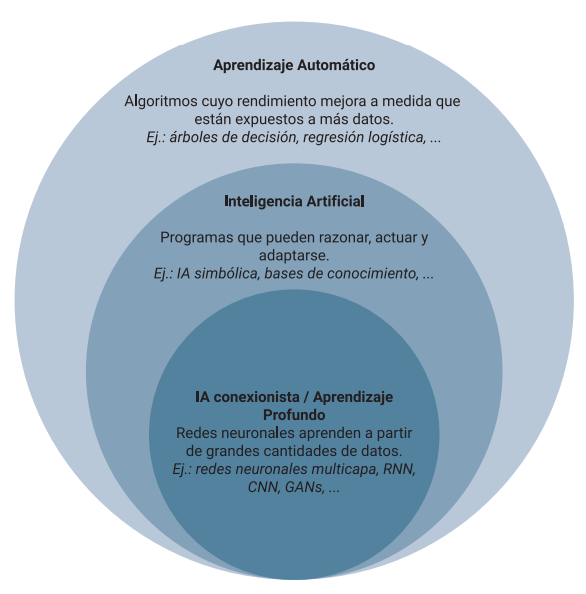
\includegraphics[width=9cm]{figs/Algoritmos de ML.png}
    \end{center}
    \caption{Diagrama de Venn de la relación entre distintas áreas de la IA}
    \label{fig:AlgoritmosML}
\end{figure}

El Machine Learning, abarca desde enfoques más superficiales hasta técnicas más avanzadas, tal y como se ha podido observar, sin embargo, es el Deep Learning lo que realmente potencia la capacidad de las máquinas para aprender y generalizar patrones complejos de manera excepcional. En la próxima sección, se hablará sobre el Deep Learning, centrándose en las RNA y en cómo estas posibilitan abordar tareas más complejas, como el reconocimiento de patrones en imágenes o el procesamiento de lenguaje natural.


\section{Deep Learning}
\label{sec:DeepLearning} 
El Deep Learning o aprendizaje profundo, constituye una rama de la IA, incluida dentro del Machine Learning, cuyos modelos computacionales se inspiran en el funcionamiento del cerebro humano y se diseñan con el propósito de adquirir conocimientos y llevar a cabo tareas específicas mediante el procesamiento de datos.\\ %La etiqueta \textit{profundo} hace referencia a la presencia de múltiples capas de neuronas artificiales en la red, lo que facilita la representación jerárquica de características y potencia la capacidad para aprender y poder diferenciar patrones complejos a partir de los datos.\\

Estas Redes Neuronales Artificiales (RNA) o Artificial Neural Networks (ANN) en inglés, están inspiradas en las redes neuronales biológicas del cerebro humano, tal y como muestra la Figura \ref{fig:Modelo neurona}, presentando características del mismo, ya que estas aprenden de la experiencia, generalizan de ejemplos previos a ejemplos nuevos, y abstraen las características principales de una serie de datos. En las RNA, la unidad análoga a la neurona biológica es el elemento procesador, PE (Process Element). Un PE tiene varias entradas y las combina, normalmente, con una suma básica. La suma de las entradas es modificada por una función de transferencia y el valor de la salida de esta función de transferencia se pasa directamente a la salida del elemento procesador. Existen dos capas con conexiones con el mundo exterior, una capa de entrada o \textit{buffer} de entrada, donde se presentan los datos a la red, y una capa o \textit{buffer} de salida que mantiene la respuesta de la red a una entrada, mientras que el resto de las capas reciben el nombre de capas ocultas \cite{Basogain08}.\\

\begin{figure} [H]
    \begin{center}
      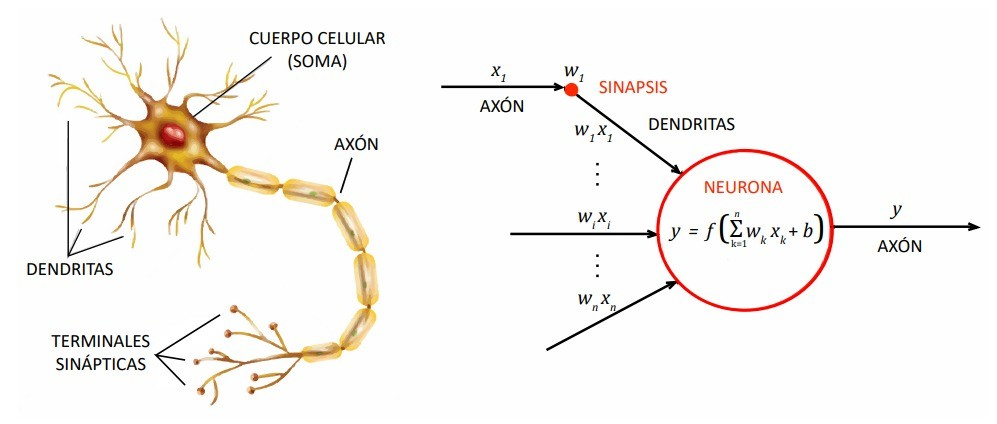
\includegraphics[width=15cm]{figs/Modelo neurona.jpeg}
    \end{center}
    \caption{Modelo biológico de una neurona genérica (izquierda) y el respectivo modelo matemático (derecha)}
    \label{fig:Modelo neurona}
\end{figure}

En consecuencia, se puede construir una red neuronal artificial mediante un conjunto de neuronas artificiales, es decir, mediante un conjunto de funciones, y conectando comúnmente la salida de cada una a las entradas de otras diferentes, como se representa en la Figura \ref{fig:Arquitectura red neuronal}. %De esta manera, las RNA no son más que redes de funciones, típicamente representadas mediante la composición de varias funciones, como se representa en la Figura \ref{fig:Arquitectura red neuronal}. Esto hace que los diferentes modelos de redes neuronales difieran principalmente en las funciones de activación utilizadas, el patrón de interconexión, e inclusive el tiempo de trasmisión de la información. 
Es importante señalar que la característica clave de la sinapsis, el escalar las señales de entrada por factores (pesos), es la manera en la que se cree que el cerebro aprende. Por lo tanto, distintos pesos dan como resultado diferentes respuestas a una entrada. De esta manera, se puede decir que el aprendizaje es el ajuste de los pesos en respuesta a un estímulo \cite{Dinamarca18}.\\

\begin{figure} [H]
    \begin{center}
      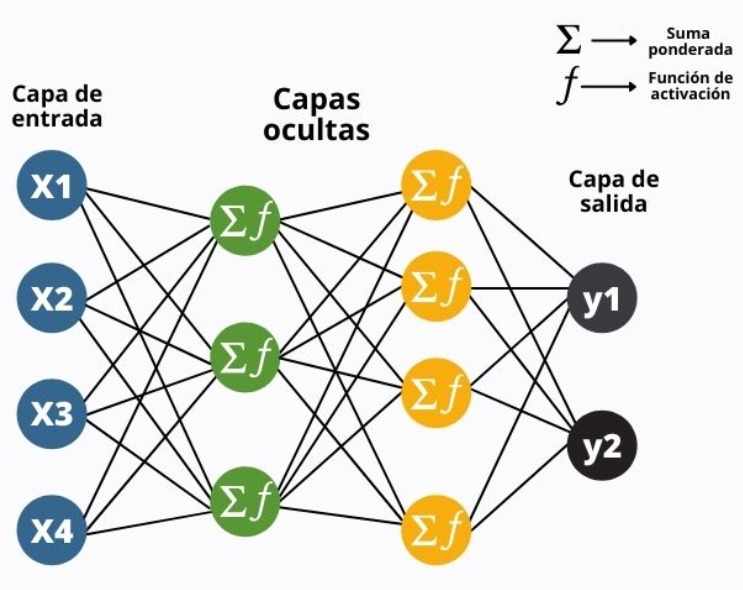
\includegraphics[width=9cm]{figs/capas rrnn.jpeg}
    \end{center}
    \caption{Arquitectura de una red neuronal}
    \label{fig:Arquitectura red neuronal}
\end{figure}

%La historia de las redes neuronales se remonta a la década de 1940, cuando el neurofisiólogo Warren McCulloch y el matemático Walter Pitts modelaron una red neuronal simple utilizando circuitos eléctricos. Su modelo estaba basado en la idea de lógica de umbral, que más tarde sería fundamental para el desarrollo de las redes neuronales artificiales. En 1958, el neurobiólogo Frank Rosenblatt dio un paso significativo al comenzar a trabajar en el perceptrón, un modelo computacional que representaba la unidad básica de una red neuronal y realizaba una suma ponderada de varias entradas, al tratarse de una unidad de procesamiento, llevando a cabo una combinación lineal de esas entradas, y aplicando posteriormente una función de activación para producir una salida. Este trabajo marcó el inicio de la investigación en redes neuronales artificiales. Saltando a la década de 2010, dos factores contribuirían a la revolución de aplicaciones de redes neuronales y algoritmos de aprendizaje profundo. En primer lugar, los avances en hardware especializado aceleraron drásticamente el entrenamiento y el rendimiento de las redes neuronales, reduciendo su consumo de energía, mientras que, en segundo lugar, el aumento de datos abiertos disponibles en línea y servicios de bajo costo para etiquetar datos impulsaron el desarrollo de la inteligencia artificial \cite{Abeliuk21}.\\

\vspace{10mm}

En este capítulo se ha introducido el nacimiento y la historia de los robots y la robótica tal y como los conocemos hoy en día, dentro de cuya rama encontramos uno de los tres grandes grupos en los cuales puede dividirse esta, la Robótica de Servicio, y para la que la Inteligencia Artificial, y más concretamente el campo de la Visión Artificial junto con el del Deep Learning, siendo este subcategoría del Machine Learning, juegan un papel fundamental en el desarrollo de nuevas aplicaciones.\\

En este proyecto se presenta un sistema que, mediante Visión Artificial y Machine Learning, es capaz de reconocer la maduración de frutos, más concretamente de fresas, con el objetivo de poder ayudar así a mejorar su proceso de recolección en un huerto vertical, gracias al algoritmo desarrollado para esto y su integración con un brazo robótico de la marca Universal Robots, que se encargará de llevar a cabo este proceso.\\
\\
\\
\\
En los siguientes capítulos de este trabajo se detallarán los objetivos del mismo, delineando claramente las metas; se expondrá la plataforma de desarrollo, detallando las herramientas seleccionadas para la elaboración del proyecto; se presentará el diseño y la arquitectura del proyecto; y, finalmente, llegaremos a las conclusiones, donde tendrá lugar una breve recopilación de información sobre los resultados obtenidos y las posibles direcciones futuras. 


\chapter{Estado del arte}
\label{cap:capitulo2}
	
En el presente capítulo, se van a describir algunos de los prototipos y soluciones más destacables aplicadas a la detección y recolección de fresas usando inteligencia artificial y técnicas robóticas.\\

\section{Descripción del problema}
\label{sec:descripcion}

Cuenta aquí el objetivo u objetivos generales y, a continuación, concrétalos mediante objetivos específicos.

\section{Requisitos}
\label{sec:requisitos}

Describe los requisitos que ha de cumplir tu trabajo.

\section{Metodología}
\label{sec:metodologia}

Qué paradigma de desarrollo software has seguido para alcanzar tus objetivos.

\section{Plan de trabajo}
\label{sec:plantrabajo}

Qué agenda has seguido. Si has ido manteniendo reuniones semanales, cumplimentando objetivos parciales, si has ido afinando poco a poco un producto final completo, etc.


\chapter{Objetivos}
\label{cap:capitulo3}
\setcounter{footnote}{12}
 
Una vez presentado el contexto general en el cual se enmarca el presente trabajo de fin de grado, en este capítulo se describen los objetivos y requisitos de este, así como la metodología y el plan de trabajo llevados a cabo.

\section{Descripción del problema}
\label{sec:descripcion}

La necesidad de implementar soluciones tecnológicas que automaticen y optimicen las tareas de recolección incrementando la eficiencia en la recolección, mejorando la calidad del producto y disminuyendo los costes asociados, surge debido a la situación actual de la agricultura en la que, uno de los mayores desafíos que enfrenta es la recolección de frutas y hortalizas, problema que deriva de la escasa mano de obra disponible y el proceso manual que esto conlleva.%, y de la posibilidad de que existan errores humanos en la identificación de los frutos para su recolección, pudiendo influenciar esto en la calidad del producto, especialmente en la recolección de frutos que requieren un manejo cuidadoso, como las fresas.\\

La solución propuesta en este trabajo busca ayudar a mejorar esta situación, proporcionando un robot de bajo coste y accesible a cualquier persona, que sirva para poder mejorar el proceso de reconocimiento por visión de la maduración de frutos, más concretamente fresas, para su posterior recolección. Por lo tanto, este proyecto pretende, como objetivo principal, utilizar un robot colaborativo que, gracias a su interfaz intuitiva sea accesible a cualquier persona y, junto con el sistema de detección elaborado con materiales de bajo coste, sea capaz de reconocer las fresas maduras de un sistema de cultivo agrícola vertical, para su posterior recolección por el brazo robótico, gracias a la comunicación establecida entre el sistema de visión y el robot.

Con el fin de alcanzar este objetivo principal, se han establecido los siguientes
subobjetivos:

\begin{enumerate}
  \item Investigar las soluciones actuales que cumplen con las características y objetivos establecidos.
  \item Seleccionar la técnica de inteligencia artificial de reconocimiento de frutas y seleccionar los componentes hardware necesarios para desarrollar el sistema de visión de bajo coste más eficiente.
  \item Optimizar la técnica escogida y adaptarla de tal manera que sea capaz de funcionar en nuestra plataforma. Al ser una técnica basada en Machine Learning, se deberá crear un dataset con imágenes de fresas y, por lo tanto, hacer un correcto tratamiento de los datos para conseguir un resultado preciso en el posterior entrenamiento.
  \item Realizar el entrenamiento con varios algoritmos de Machine Learning de
clasificación. Estudiar el rendimiento y precisión de cada uno de ellos a través de pruebas con el sistema de visión y fresas reales.
  \item Seleccionar el protocolo de comunicación entre el sistema de visión y el robot y llevar a cabo pruebas; tanto simuladas, a través del simulador que facilita el fabricante del robot, como reales, para establecer esta comunicación.
  \item Dar soporte software al robot mediante un %Programación tanto del robot como del archivo en Python que posee el código del 
sistema de reconocimiento de fresas, que guarde las posiciones y la distancia de estas a la posición de la cámara, para su posterior envío al brazo robótico.
  \item Realizar pruebas de la aplicación final, tanto en entornos simulados como reales.
\end{enumerate} 
 
\section{Plan de trabajo}
\label{sec:plantrabajo}
El desarrollo y seguimiento que el proyecto ha seguido es una planificación en base a reuniones semanales con el tutor, en las cuales se revisaron los avances, se fijaron nuevos objetivos y se discutieron y propusieron posibles mejoras, mientras que el trabajo se organizó en varias fases clave: 
\begin{enumerate}
  \item \textit{Investigación inicial:} En esta fase, se investigó el estado del arte relacionado con sistemas de visión artificial y técnicas de reconocimiento de objetos, especialmente aplicadas a la maduración de frutas y hortalizas, y utilizando para ello artículos científicos, capítulos de libros y proyectos previos. 
  \item \textit{Diseño y desarrollo del sistema de visión artificial:} Esta fase se centró en el diseño y la implementación del sistema de visión artificial, abarcando tanto el desarrollo del software como la integración del hardware, e incluyendo la calibración y obtención de los parámetros intrínsecos a la cámara y las diversas pruebas realizadas con distintos sistemas y códigos, hasta seleccionar el \textit{software} funcional con el que se llevó a cabo el proyecto finalmente.
  \item \textit{Pruebas en entorno simulado:} Durante esta fase se realizaron múltiples pruebas y ajustes para optimizar el funcionamiento del sistema y comprobar su funcionamiento en diferentes escenarios, simulando de manera separada la programación del robot, para el que se utilizó un simulador en una máquina virtual, y la detección y funcionamiento del sistema de visión, cuyos algoritmos se afinaron para mejorar la precisión en la detección y se ajustaron los parámetros relacionados con la cámara en los códigos para poder obtener las coordenadas y distancia real de las detecciones respecto a la cámara y poder transmitírselas al brazo robótico. Finalmente, también se llevaron a cabo pruebas de comunicación entre el sistema de visión y el robot, poniendo a prueba su programación, para que este alcanzase el punto de la detección.
  \item \textit{Pruebas en entorno real:} Una vez desarrollado el prototipo inicial, el sistema completo fue sometido a pruebas en un entorno real de lo que sería la aplicación final. 
  \item \textit{Escritura de la memoria:} Con el sistema ya afinado y probado, se procedió a la redacción de la memoria del proyecto. En esta etapa, se documentó detalladamente todo el proceso seguido, desde la investigación inicial hasta los resultados finales obtenidos durante las pruebas reales. 
\end{enumerate}


Todo el contenido del proyecto se puede encontrar en un repositorio público de GitHub\footnote{\url{https://github.com/RoboticsURJC/tfg-dcampoamor}}, en cuya wiki\footnote{\url{https://github.com/RoboticsURJC/tfg-dcampoamor/wiki}} se puede ver el desarrollo del trabajo en semanas a lo largo de los meses, durante el trascurso del proyecto. Las requisitos necesarios para la consecución de los objetivos planteados, las competencias desarrolladas y la metodología empleada pueden encontrarse descritos en el Anexo \ref{cap:capitulo7}.
%Después de haber revisado los objetivos, requisitos, competencias, metodología y el plan de trabajo implementado para la realización de este proyecto, en el siguiente capítulo se abordarán las plataformas de desarrollo empleadas.



\chapter{Plataforma de desarrollo}
\label{cap:capitulo4}
 
Con los objetivos del proyecto definidos, en este capítulo se abordarán las distintas plataformas de desarrollo, tanto \textit{hardware} como \textit{software}, que han facilitado el logro de esos objetivos.

\section{Hardware}
\label{sec:hardware}

Este apartado recoge la descripción de los componentes \textit{hardware} utilizados en este proyecto, para los cuales se ha buscado priorizar la reducción de costes en cada elección y utilizar aquellos elementos a los que se tenía acceso al desarrollar el proyecto.

\subsection{Cámara Logitech C270 HD}
\label{subsec:logiC270HD}

Esta cámara web (Figura \ref{fig:logiC270HD}) de dimensiones 72,91 x 31,91 x 66,64 mm, corrige la iluminación de manera automática, produciendo colores reales y naturales y ajustándose a las condiciones de iluminación del entorno, lo que facilita la detección de fresas. Ofrece una resolución HD 720p, proporcionando imágenes claras y nítidas a una velocidad de 30 fotogramas por segundo (fps), con una lente que cuenta con enfoque fijo y un campo visual diagonal (dFoV) de 55 grados. Su coste aproximado es de entre 30-40€.

\begin{figure} [H]
    \begin{center}
      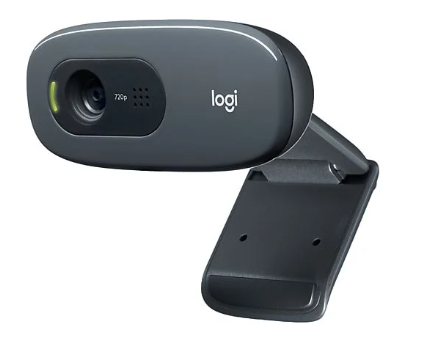
\includegraphics[width=5cm]{figs/logi C270.png}
    \end{center}
    \caption{Cámara Logitech C270 HD$^{\ref{note:enlace16}}$}
    \label{fig:logiC270HD}
\end{figure}

\setcounter{footnote}{16}
\footnotetext[\value{footnote}]{\url{https://www.logitech.com/es-es/products/webcams/c270-hd-webcam.960-001063.html?srsltid=AfmBOor4HptUTcGrxE-4SZxKR-ARw-ykNeagHSEzXUvTlXkx8qLfY4lG}\label{note:enlace16}}

\subsection{Soporte de brazo articulado}
\label{subsec:soporte_camara}

Para poder ubicar la cámara en una posición fija desde la cual visualizar las fresas, se utilizó un soporte de brazo articulado (Figura \ref{fig:soporte_camara}), cuya parte fija en la parte inferior se ancla a la mesa. Este soporte articulado tiene un ajuste de 360 grados, con su extremo más largo de 75 cm, mientras que la carga máxima que permite es de 560 gramos cuando se coloca de manera horizontal, siendo el precio de este soprte 22,98€.

\begin{figure} [H]
    \begin{center}
      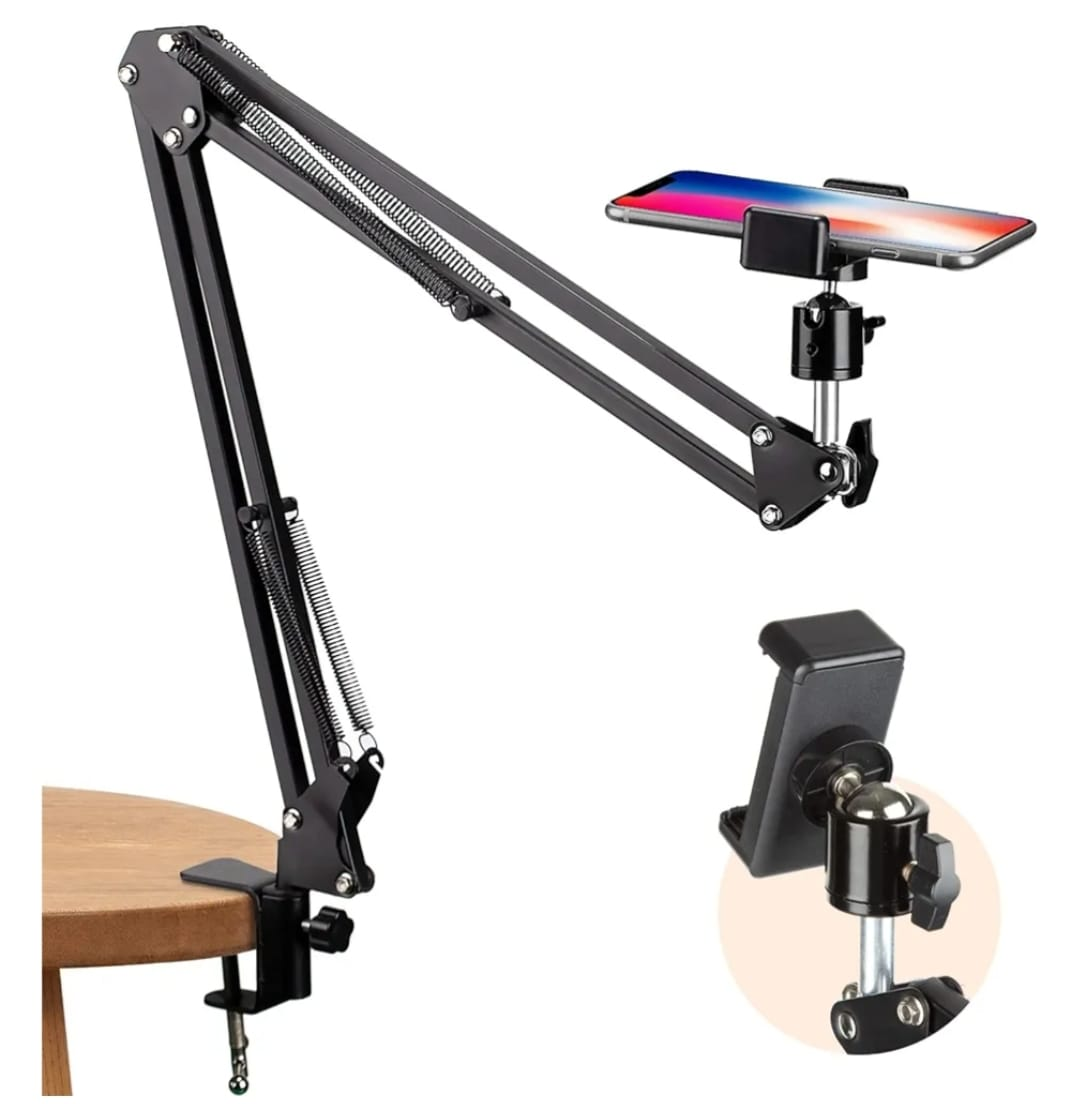
\includegraphics[width=5cm]{figs/Soporte de brazo articulado.jpeg}
    \end{center}
    \caption{Soporte de brazo articulado$^{\ref{note:enlace17}}$}
    \label{fig:soporte_camara}
\end{figure}
 
\setcounter{footnote}{17} 
\footnotetext[\value{footnote}]{\url{https://www.amazon.es/dp/B08JCG4V5S?ref=ppx_pop_mob_ap_share&th=1}\label{note:enlace17}}

\subsection{Ordenador principal}
\label{subsec:ordenador}

El equipo que se ha configurado como entorno de trabajo para este proyecto es el que aparece en la Figura \ref{fig:PC_Lenovo}, sirviendo como base para el desarrollo de la programación y las pruebas de la visión artificial, y utilizándose igualmente como servidor para poder llevar a cabo la comunicación con el brazo robótico mediante el protocolo XML-RPC basado en HTTP, y posteriormente el envío de posiciones detectadas en tiempo real a este. 

\begin{figure} [H]
    \begin{center}
      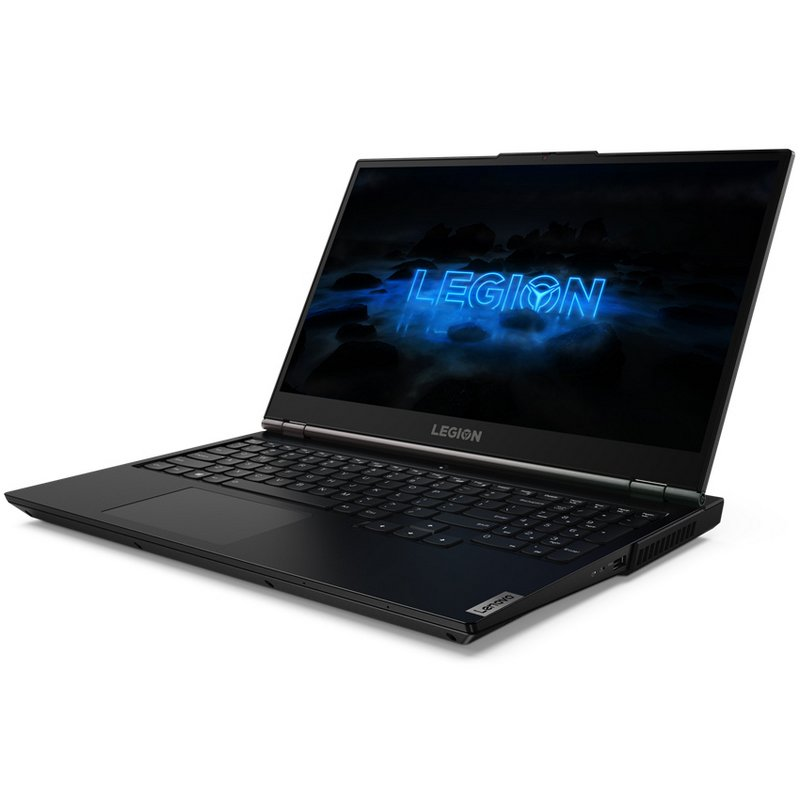
\includegraphics[width=7cm]{figs/Lenovo Legion 5 15imh05.jpg}
    \end{center}
    \caption{Lenovo Legion 5 15IMH05$^{\ref{note:enlace18}}$}
    \label{fig:PC_Lenovo}
\end{figure}

\setcounter{footnote}{18}
\footnotetext[\value{footnote}]{%
    https://www.pccomponentes.com/lenovo-legion-5-15imh05-intel-core-i7-10750h-16gb-1tb-ssd-gtx-1650-156?srsltid=AfmBOopJpvGSHUyQU696jgG7-6orSKMOEWZe2ZvvYtA0NGtJ9Ms2xJFp%
    \label{note:enlace18}%
}
    
A continuación, en el Cuadro \ref{cuadro:carac_ordena}, se recogen las características técnicas del ordenador utilizado:

\begin{table}[H]
	\begin{center}
		\begin{tabular}{|c|c|}
			\hline
			\textbf{Características} & \textbf{Descripción} \\
			\hline
			\multirow{2}{*}{Pantalla} & \multirow{2}{*}{\shortstack{15,6 pulgadas \\ Full HD (1920x1080)}} \\
			& \\
			\hline
			Procesador (CPU) & Intel Core i7-10750H CPU @ 2.60GHz \\
			\hline
			Memoria RAM & 16 GB \\
			\hline
			Almacenamiento & 1 TB \\
			\hline
			Tarjeta gráfica (GPU) & NVIDIA GeForce GTX 1650 Ti Mobile \\
			\hline
			Sistema Operativo & Windows 10 y Ubuntu 22.04.4 LTS \\
			\hline
			Cámara de portátil & HD 720p con tapa de privacidad \\
			\hline
			\multirow{5}{*}{Puertos} & \multirow{5}{*}{\shortstack{4 x USB 3.2 Gen 1 Tipo-A \\ 1 x USB 3.2 Gen 1 Tipo-C \\ 1 x Ethernet (RJ-45) \\ 1 x HDMI 2.0 \\ 1 x combo auriculares/micrófono (3.5 mm)}} \\
			& \\
			& \\
			& \\
			& \\
			\hline
			Conectividad & WiFi 6 802.11ax (2x2), Bluetooth 5.0, Ethernet 100/1000M \\
			\hline
			Batería & 80 Wh \\
			\hline
			Peso & 2,3 kg \\
			\hline
			Dimensiones & 363,06 x 259,61 x 23,57--26,1 mm \\
			\hline
		\end{tabular}
		\caption{Especificaciones técnicas del ordenador usado}
		\label{cuadro:carac_ordena}
	\end{center}
\end{table}

\subsection{Robot de \textit{Universal Robots} de la gama \textit{e-series}}
\label{subsec:URe-series}

Los robots de Universal Robots, también conocidos como robots colaborativos o cobots, están diseñados para trabajar junto a los humanos de manera segura, eficiente y flexible tanto en aplicaciones industriales como no industriales, destacando por su facilidad de uso, versatilidad y capacidad para automatizar tareas repetitivas o peligrosas \cite{UR_e-series_brochure18}. 

Fabricados en aluminio junto con otros materiales de bajo peso, %permitiendo reducir la inercia del propio robot y facilitar su manipulación, 
cada brazo robótico tiene seis ejes, otorgando al robot seis grados de libertad (Degree Of Freedom o DOF), que permiten movimientos precisos y fluidos, y en cuyas articulaciones están equipadas, a su vez, encoders absolutos, reductoras armónicas, que reducen la velocidad de rotación de los engranajes en las juntas, y aumentan el par del eje, ofreciendo una alta precisión y eficiencia; y, en aquellos brazos robóticos pertenecientes a la gama e-series, sensores de fuerza y torque, encontrándose integrados en el efector o tool flange del propio brazo robótico\footnote{\url{https://www.universal-robots.com/mx/acerca-de-universal-robots/noticias/meet-the
-next-generation-of-collaborative-ur-robots-at-robobusiness}}. 

%Por otro lado, en la controladora de los brazos robóticos de la gama e-series, pueden diferenciarse varios módulos \cite{Service_Manual_UR_e-series_2024}: 

%\begin{itemize}
%    \item Unidad de procesamiento principal (CPU): que se encarga de realizar los cálculos cinemáticos y dinámicos del robot, la ejecución de programas y control del brazo robótico mediante su software Polyscope, junto con la comunicación con los periféricos y la consola de mando o teach pendant.
%    \item Fuente de alimentación: que suministra energía a todos los componentes del sistema, incluyendo a las articulaciones del brazo robótico y el teach pendant, y que incluye protección contra sobrecargas y cortocircuitos para garantizar una alimentación estable y segura.
%    \item Módulo de seguridad o la placa de seguridad (Safety Control Board o SCB): que implementa funciones de seguridad colaborativa, como límites de velocidad, fuerza y espacio de trabajo, y que supervisa las entradas de seguridad y gestiona las paradas de emergencia.
%    \item Interfaces de comunicación: compuesta del puerto ethernet, que soporta los protocolos de comunicación TCP/IP, ModbusTCP, ProfiNet y EthernetIP,  los dos puertos USB (uno de ellos USB 2.0 y otro USB 3.0), las dieciseis entradas y salidas digitales, y las dos entradas y salidas analógicas.
%    \item Sistema de refrigeración: compuesto por ventiladores internos, que están controlados por sensores térmicos que ajustan su velocidad en función de la temperatura interna de los componentes, llegando a activar alarmas si se detectasen temperaturas anormales, rejillas de ventilación en el lateral de la carcasa o envolvente de acero que recubre y protege los componentes internos de la controladora, que a su vez están protegidas por filtros para evitar la entrada de polvo o partículas grandes. 
%    \item Módulo de almacenamiento interno: espacio dedicado para guardar y almacenar el sistema operativo basado en Linux y el software de la interfaz gráfica y entorno de programación del robot llamado Polyscope, programas, configuraciones, y datos operativos del robot como registros de eventos de datos de diagnóstico. Para esta gama de robots se utiliza una tarjeta SD de almacenamiento interno.
%\end{itemize}

Para el desarrollo de este proyecto se han utilizado diferentes modelos de robots de la gama e-series, todos ellos representados en la Figura \ref{fig:Gama_e-series}, desde el UR3e \cite{User_Manual_UR3e_2025} hasta el UR10e \cite{User_Manual_UR10e_2025}, pasando por el UR5e  \cite{User_Manual_UR5e_2025} .
A pesar de que tanto la gama CB-series como la gama e-series permiten la comunicación mediante el protocolo XML-RPC, la interfaz más intuitiva y simplificada que facilita la programación y reduce la sobrecarga de información, poseer sensor de fuerza integrado, permitiendo un control más preciso y sensible haciendo que mejore la interacción con el entorno, así como una mayor precisión en la repetición de movimientos, entre otros factores, constituyeron que se eligiera la gama e-series para este trabajo \cite{Service_Manual_UR_e-series_2024}.

\begin{figure} [H]
    \begin{center}
      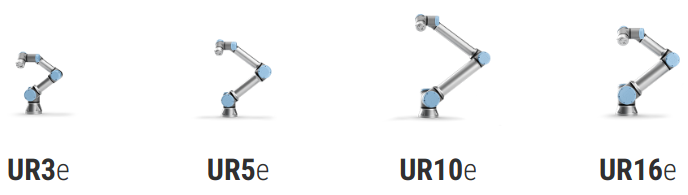
\includegraphics[width=16cm]{figs/Gama e-series.png}
    \end{center}
    \caption{Gama e-series de Universal Robots$^{\ref{note:enlace20}}$}
    \label{fig:Gama_e-series}
\end{figure}

\setcounter{footnote}{20} 
\footnotetext[\value{footnote}]{\url{https://www.universal-robots.com/es/productos/}\label{note:enlace20}}


\subsection{Comunicaciones}
\label{subsec:comunicacion}

En este proyecto, la comunicación entre el robot y el ordenador que ejecuta el servidor XML-RPC se establece vía Ethernet, permitiendo una conexión rápida y confiable. La infraestructura de red juega un papel fundamental en esta comunicación, ya que el robot y el servidor deben estar correctamente configurados dentro de la misma red, por lo que se emplea un switch Ethernet, en este caso el TP-Link LS105G %(Figura \ref{fig:TPLink_LS105G})
, para gestionar las conexiones entre los diferentes dispositivos y asegurar una comunicación fluida y sin interferencias.

Este switch de escritorio, cuyo precio es de 14,90€,  posee cinco puertos Ethernet RJ45 a 10/100/1000 Megabits por segundo (Mbps), permitiendo la transferencia instanténea de archivos y paquetes, con gran ancho de banda y sin interferencias, y no necesita configuración manual previa, ya que se trata de un dispositivo \emph{plug and play}, por lo que simplemente se tiene que conectar y empieza a funcionar. 

%\begin{figure} [H]
%    \begin{center}
%      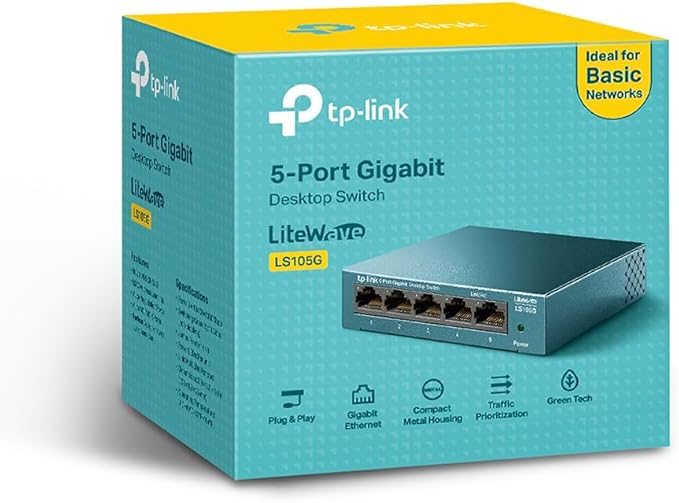
\includegraphics[width=6cm]{figs/TPLink LS105G.jpg}
%    \end{center}
%    \caption{Switch TP-Link LS105G$^{\ref{note:enlace21}}$}
%    \label{fig:TPLink_LS105G}
%\end{figure}

\setcounter{footnote}{21} 
\footnotetext[\value{footnote}]{\url{https://www.tp-link.com/es/business-networking/litewave-switch/ls105g/}\label{note:enlace21}}

\section{Software}
\label{sec:software}

Este apartado estará dedicado a detallar las plataformas de software, librerías y entornos de trabajo que han sido fundamentales para alcanzar los objetivos definidos en el Capítulo 3, desde el sistema operativo utilizado hasta las tecnologías específicas para el procesamiento de imágenes y aprendizaje profundo.

\subsection{Ubuntu}
\label{sec:ubuntu}
Ubuntu\footnote{\url{https://ubuntu.com/}} es un sistema operativo de código abierto basado en Linux y desarrollado por la empresa británica Canonical Ltd. 
Este sistema operativo está diseñado para ser utilizado en una gran variedad de dispositivos, y es reconocido por su facilidad de uso, estabilidad y seguridad, contando con una amplia comunidad de desarrolladores y usuarios que contribuyen activamente a su desarrollo y soporte. La versión utilizada para la realización de este proyecto, de entre todas las versiones disponibles, es Ubuntu 22.04 Long Term Support (LTS) (Jammy Jellyfish), ya que era la última versión disponible de Ubuntu en el momento en el que se empezó a elaborar el proyecto. 

\subsection{Polyscope}
\label{sec:Polyscope}

Polyscope\footnote{\url{https://www.universal-robots.com/es/productos/polyscope/}} es la interfaz de usuario gráfica desarrollada por Universal Robots para poder programar y utilizar sus robots colaborativos. Está diseñada para ser intuitiva y accesible, ya que permite a los usuarios crear programas de robot sin necesidad de conocimientos avanzados en programación. 

Construido sobre una plataforma basada en Linux, PolyScope está basado en una arquitectura de software que combina una interfaz gráfica amigable con un lenguaje de programación propio llamado URScript, permitiendo tanto a usuarios sin experiencia en programación como a programadores avanzados interactuar eficazmente con los robots UR, ya que la interfaz gráfica facilita la creación de programas mediante bloques visuales, mientras que URScript ofrece una mayor flexibilidad para desarrollos más complejos.

A lo largo de los años, Universal Robots ha lanzado varias versiones de PolyScope, cada una con mejoras y nuevas funcionalidades, siendo la primera versión PolyScope 3, lanzada en 2012, ya que fue diseñada para la serie CB3 de robots UR. PolyScope 5\footnote{\url{https://www.universal-robots.com/products/polyscope-5/}} (Figura \ref{fig:Polyscope5}) se introdujo en junio de 2018, coincidiendo con el lanzamiento de la gama de robots e-series de Universal Robots. Por último, PolyScope X\footnote{\url{https://www.universal-robots.com/products/polyscope-x/}} es la última evolución del software de Universal Robots, siendo su lanzamiento oficial en noviembre de 2024\footnote{\url{https://www.universal-robots.com/2024q3/polyscope-x-festival/}}, y estando basado en tecnologías como ROS2 y contenedores Docker, centraliza las funciones más importantes y simplifica la programación mediante el uso de plantillas predefinidas. %, incluyendo mejoras respecto a Polyscope 3 en la interfaz de usuario (Figura \ref{fig:Polyscope5}), haciéndola más intuitiva y moderna y facilitando la programación y configuración del robot, incluyendo nuevas funcionalidades de seguridad como la capacidad de restringir la entrada de una esfera virtual en una zona o plano de seguridad y establecer límites de velocidad y distancia de frenado mejorando la seguridad en el entorno de trabajo; incrementando la frecuencia de control a 500 hercios (Hz) permitiendo de esta manera movimientos más precisos e incorporando soporte para nuevas características de hardware como la interfaz de comunicación de herramientas (Tool Communication Interface) en la que el conector de herramientas puede utilizarse para la comunicación serie RS485 con una velocidad de datos de hasta 5 megabits\footnote{\url{https://forum.universal-robots.com/t/release-of-e-series-polyscope-5-0-polyscope-3-6-sdk-1-3-and-a-brand-new-developer-community}}.

\begin{figure} [H]
    \begin{center}
      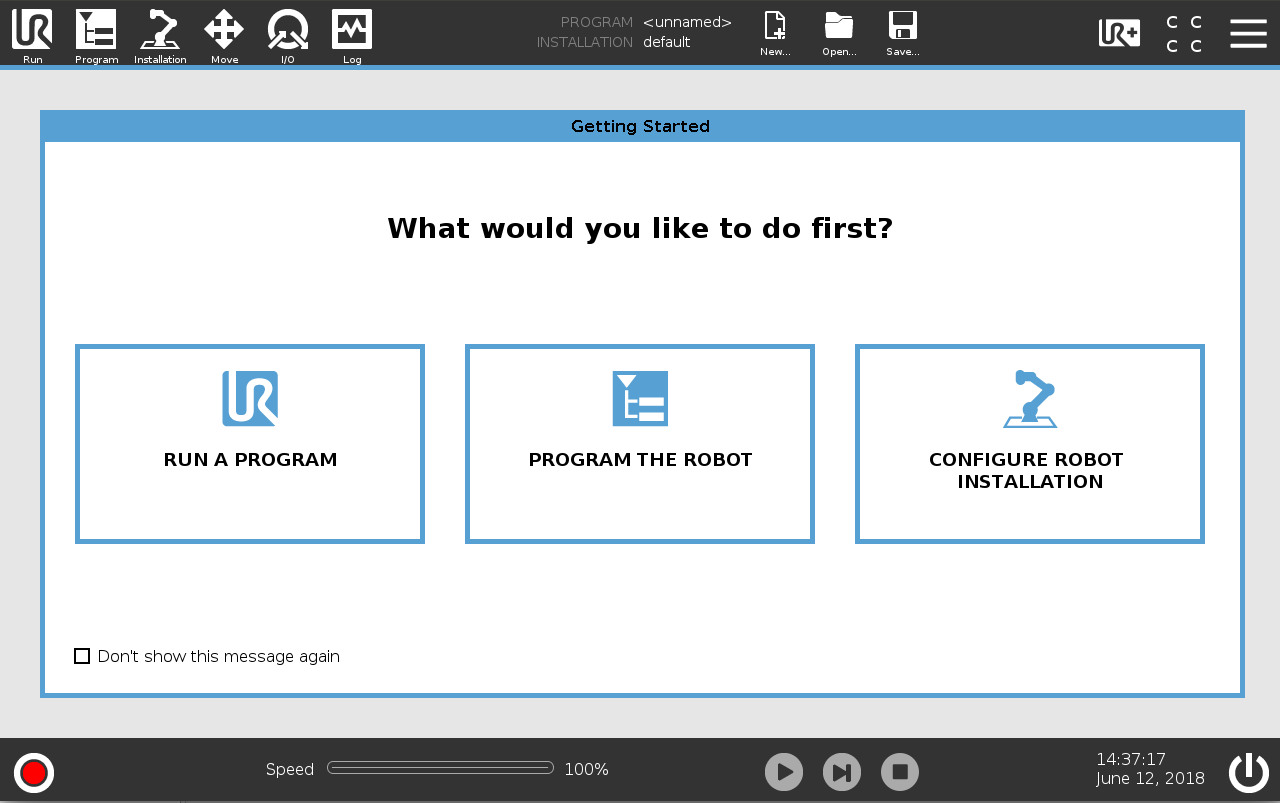
\includegraphics[width=15cm]{figs/InterfazPolyscope5.png}
    \end{center}
    \caption{Pantalla principal de la interfaz de Polyscope 5}
    \label{fig:Polyscope5}
\end{figure}

%Por último, PolyScope X\footnote{\url{https://www.universal-robots.com/products/polyscope-x/}} es la última evolución del software de Universal Robots, diseñado para simplificar y potenciar los procesos de automatización, %Aunque se presentó un prototipo en la feria International Manufacturing Technology Show (IMTS) en 2022 y se mostró en Automatica en Múnich en junio de 2023, siendo su lanzamiento oficial en noviembre de 2024\footnote{\url{https://www.universal-robots.com/2024q3/polyscope-x-festival/}}. Basado en tecnologías como ROS2 y contenedores Docker, ofrece una plataforma más flexible y escalable para el desarrollo y la integración de aplicaciones,%modificando de nuevo la interfaz de usuario (Figura \ref{fig:PolyscopeX}) respecto a Polyscope 5, centralizando las funciones más importantes y simplificando la programación mediante el uso de plantillas predefinidas. %para agilizar y facilitar la creación de módulos reutilizables y simplificando la programación a los operarios, reduciendo de esta manera la complejidad en el desarrollo de aplicaciones.

%\begin{figure} [H]
%    \begin{center}
%      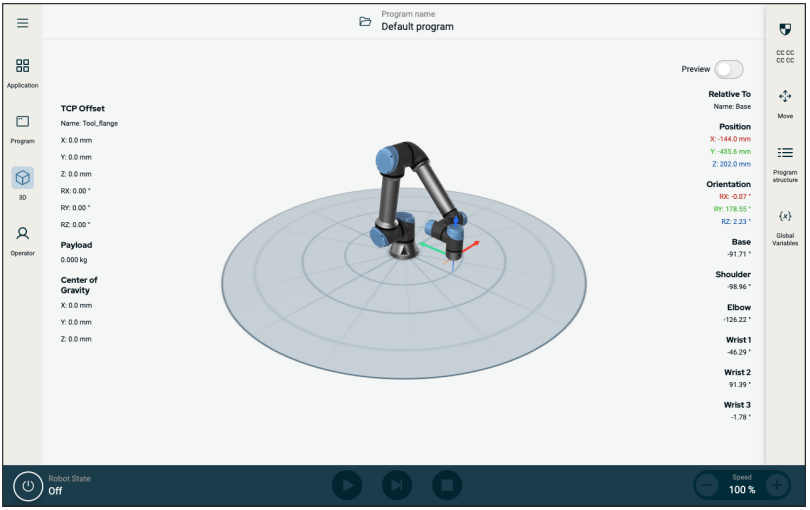
\includegraphics[width=13cm]{figs/InterfazPolyscopeX.png}
%    \end{center}
%    \caption{Pantalla principal de la interfaz de Polyscope X}
%    \label{fig:PolyscopeX}
%\end{figure}

A pesar de que Polyscope X es compatible con los robots de la gama e-series, se deben cumplir una serie de requisitos en cuanto al hardware de la controladora para poder actualizar desde Polyscope 5, por lo que para el desarrollo de este proyecto se ha terminado utilizado la versión 5.16 de Polyscope 5, puesto que no se cumplían todos los requisitos para que se diera esta actualización en los robots utilizados.

\subsection{Python}
\label{sec:python}
Python\footnote{\url{https://www.python.org/}} es un lenguaje de programación de alto nivel, orientado a objetos y de semántica dinámica. La sintaxis de Python, sencilla y fácil de aprender, favorece la legibilidad y, por tanto, reduce el coste de mantenimiento de los programas, admitiendo módulos y paquetes, lo que fomenta la modularidad del programa y la reutilización de código \footnote{\url{https://www.python.org/doc/essays/blurb/}} para el desarrollo de aplicaciones en diferentes áreas, como sucede en este caso con la inteligencia y visión artificial y el aprendizaje automático. 
\pagebreak

\subsection{PyTorch}
\label{sec:PyTorch}

De los desarrolladores de Facebook AI Research junto a otros laboratorios, PyTorch\footnote{\url{https://pytorch.org/}} es un marco de aprendizaje profundo de código abierto conocido por su compatibilidad con Python, siendo un marco de trabajo completo para crear modelos de aprendizaje profundo. Se distingue por su excelente compatibilidad con GPU y su uso de la autodiferenciación en modo inverso, que permite modificar los gráficos de cálculo sobre la marcha, lo que lo convierte en una opción popular para la experimentación rápida y la creación de prototipos.

\subsection{NumPy}
\label{sec:NumPy}

NumPy (Numerical Python)\footnote{\url{https://numpy.org/}} es una biblioteca de Python fundamental para el cálculo numérico, que proporciona un objeto de matriz multidimensional, varios objetos derivados (como matrices y matrices enmascaradas) y un surtido de rutinas para realizar operaciones rápidas con matrices \footnote{\url{https://numpy.org/doc/stable/user/whatisnumpy.html/}}. 

En este proyecto, la biblioteca Numpy se ha utilizado para inicializar matrices y vectores de los parámetros intrínsecos y extrínsecos de la cámara, realizar cálculos geométricos y poder obtener las matrices de rotación y traslación de la cámara, llevar a cabo operaciones matriciales como multiplicaciones e inversiones, y para poder proyectar las coordenadas en el espacio 2D a coordenadas tridimensionales mediante operaciones matriciales, pudiendo obtener posteriormente las distancias a los objetos detectados. 

\subsection{OpenCV}
\label{sec:OpenCV}

OpenCV (Open Source Computer Vision Library)\footnote{\url{https://opencv.org/}} es una biblioteca de software de código abierto diseñada para su uso en aplicaciones de aprendizaje automático y visión artificial. Desarrollado por Intel \footnote{\url{https://www.intel.es}} en 1999, cuenta con más de 2.500 algoritmos optimizados, que incluyen un amplio conjunto de algoritmos de visión por ordenador y aprendizaje automático.%, que permiten desde el reconocimiento y detección de caras, objetos y acciones humanas en vídeos, hasta el seguimiento de movimientos de estos a tiempo real en vídeo. Además, incluyen herramientas para la creación de modelos y nubes de puntos 3D, la generación de imágenes de alta resolución a partir de múltiples tomas, y la búsqueda de imágenes similares en bases de datos. También ofrecen funcionalidades como la eliminación de ojos rojos, el seguimiento ocular, el reconocimiento de paisajes, y la superposición de realidad aumentada mediante marcadores.

En este proyecto, OpenCV (importado como cv2) se ha usado para poder capturar los frames desde la cámara en tiempo real y mostrarlo en una ventana para poder controlar y verificar que se realizan las detecciones correctamente, para convertir estos frames del formato BGR a RGB, dibujar un rectángulo alrededor de las fresas detectadas, añadiendo la etiqueta de texto correspondiente que indica la clase detectada y la confianza de esta detección; permite detener el bucle principal del programa, terminarlo y salir de este si se presiona la tecla configurada para ello, asegurando que la cámara o el archivo de vídeo no permanezcan bloqueados por el programa y cerrando todas las ventanas de visualización creadas.

\subsection{XML-RPC}
\label{sec:XMLRPC}

XML-RPC\footnote{\url{https://docs.python.org/es/3.8/library/xmlrpc.html}} es un método de llamada a procedimiento remoto (RPC) que usa XML para codificar y tranferir datos entre programas a través de sockets y HTTP como protocolo de transporte. Para muchos lenguajes de programación existen servidores XML-RPC gratuitos, entre otros para: Python, Java, C++ y C.

Debido al uso de Python en el proyecto, se utilizó el paquete \textit{xmlrpc}, que agrupa los módulos tanto de cliente como de servidor que implementan XML-RPC. Con este paquete, el controlador del robot UR puede llamar a métodos o funciones (con parámetros) en un programa/servidor remoto y obtener de vuelta datos estructurados, pudiendo realizar un cálculo complejo mediante su uso, que no está disponible en el lenguaje propio de programación del robot.

\subsection{Anaconda}
\label{sec:Anaconda}

Anaconda\footnote{\url{https://www.anaconda.com/}} es una distribución de código abierto para los lenguajes de programación Python y R, diseñada para facilitar la gestión de paquetes y entornos, así como el despliegue de aplicaciones de ciencia de datos y aprendizaje automático. Ofrece herramientas como conda, un sistema de gestión de paquetes y entornos que funciona en Windows, macOS y Linux; y Anaconda Navigator, una aplicación de escritorio que permite gestionar aplicaciones integradas, paquetes y entornos sin necesidad de utilizar la línea de comandos\footnote{\url{https://docs.anaconda.com/anaconda/}}. 

Para este proyecto se ha hecho uso del programa Conda, ya que, utilizando esta herramienta es posible instalar y actualizar paquetes y dependencias y cambiar entre entornos desde el mismo ordneador local, permitiendo que puedan ser mantenidos y ejecutados independientemente sin archivos, directorios y rutas, para que se pueda trabajar con versiones específicas de librerías y/o Python mismo, sin afectar a otros proyectos Python, es decir, no afectando los cambios de un entorno a otros \footnote{\url{https://docs.anaconda.com/reference/glossary/\#conda}}.

\subsection{YOLOv3}
\label{sec:YOLOv3}

YOLOv3 (You Only Look Once versión 3)\footnote{\url{https://docs.ultralytics.com/es/models/yolov3/}} es un algoritmo de detección de objetos en tiempo real que identifica y localiza múltiples objetos dentro de una imagen o video. Desarrollado por Joseph Redmon y Ali Farhadi en 2018, YOLOv3 es la tercera iteración de la serie YOLO, conocida por su capacidad para realizar detecciones rápidas y precisas \cite{Redmon18}. %Introdujo el uso de tres escalas diferentes para la detección, aprovechando tres tamaños distintos de núcleos de detección: 13x13, 26x26 y 52x52, lo que mejoró significativamente la precisión de la detección de objetos de diferentes tamaños \footnote{\url{https://docs.ultralytics.com/es/models/yolov3/\#key-features}}. 
La serie YOLOv3, está diseñada específicamente para tareas de detección de objetos, además, YOLOv3 añadió funciones como predicciones multietiqueta para cada cuadro delimitador y una red extractora de características mejorada. Estos modelos son famosos por su eficacia en diversos escenarios del mundo real, equilibrando precisión y velocidad, lo que los hace adecuados para una amplia gama de aplicaciones \footnote{\url{https://docs.ultralytics.com/es/models/yolov3/\#supported-tasks-and-modes}}.\\

Esta herramienta ha sido elegida para el entrenamiento del modelo de detección de fresas debido a su eficiencia en el uso de recursos computacionales, lo que lo hace más accesible para sistemas con capacidades limitadas; a la amplia documentación y la comunidad activa existente en torno a YOLOv3, que proporciona recursos valiosos para la implementación y resolución de problemas, lo que es esencial en proyectos académicos con plazos definidos \footnote{\url{https://github.com/ultralytics/yolov3/}}; a la competencia en cuanto a precisión y velocidad de YOLOv3 frente a versiones superiores a pesar de presentar estas ciertas mejoras; y a que YOLOv3 es compatible con entornos de desarrollo ampliamente utilizados en proyectos académicos, como Python y bibliotecas estándar de aprendizaje automático, facilitando su integración en el flujo de trabajo del proyecto.

\vspace{20mm}

Una vez analizadas las plataformas de software y hardware utilizadas en este trabajo de fin de grado, se procederá a detallar el proceso completo de diseño y desarrollo de la aplicación, lo cual será explicado con detalle en los capítulos siguientes.








\chapter{Descripción del sistema}
\label{cap:capitulo5}

%La automatización de tareas agrícolas mediante tecnologías de visión artificial es una línea de investigación en plena expansión, especialmente en lo que respecta a la cosecha de productos delicados como las frutas, y más concretamente, las fresas. La maduración irregular, la variabilidad del entorno y la necesidad de recolección selectiva representan retos importantes, por lo que este proyecto nace con el propósito de aportar una solución basada en visión artificial y robótica colaborativa que permita mejorar la eficiencia y precisión en la recolección, reduciendo la intervención humana y el riesgo de daños al fruto.\\

%El presente Trabajo de Fin de Grado se enmarca en el desarrollo de un sistema de visión por ordenador para la detección de fresas maduras, con el objetivo de facilitar su recolección mediante un brazo robótico de la marca Universal Robots (UR). Este sistema propuesto permite detectar visualmente las fresas y estimar su posición en el espacio tridimensional utilizando una única cámara, integrando los datos en tiempo real con el robot colaborativo para ejecutar tareas de recolección automática.

Una vez expuestos el estado del arte, los objetivos del proyecto y las plataformas de desarrollo empleadas, en este capítulo se describe de forma detallada el sistema en su conjunto (Figura \ref{fig:montaje_final}), y se abordan tanto los fundamentos teóricos que lo sustentan como el proceso seguido para su diseño e implementación, con el objetivo de ofrecer una visión completa del funcionamiento del sistema.

\begin{figure} [H]
    \begin{center}
      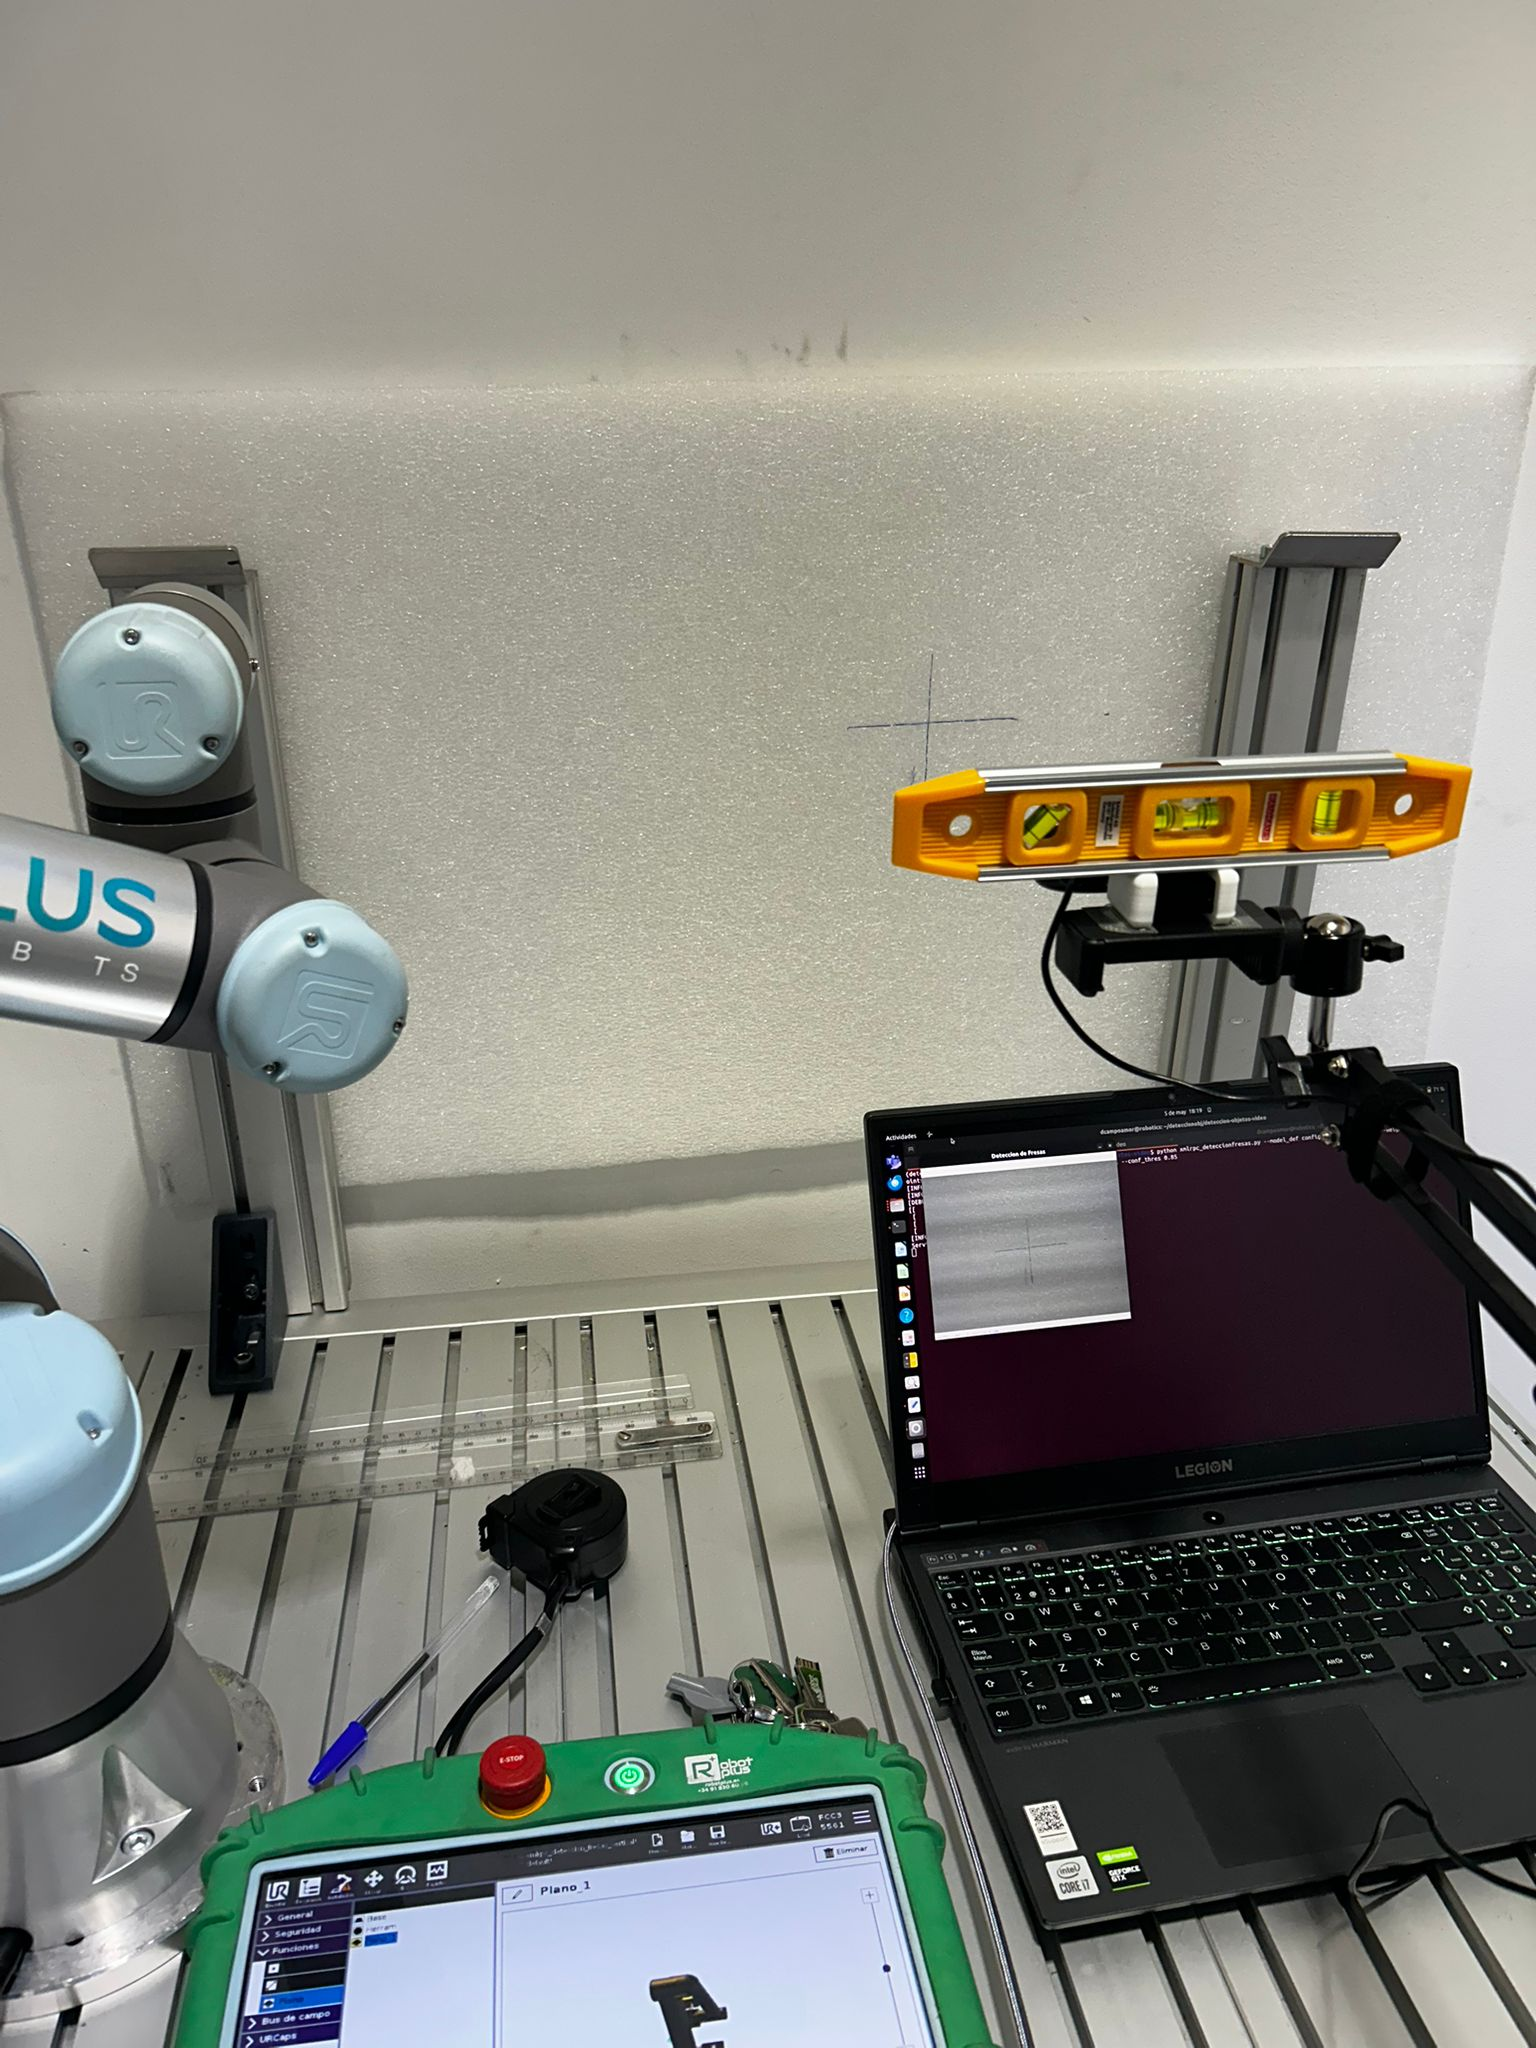
\includegraphics[width=9cm]{figs/Set up coordenadas pruebas plano vertical UR5e_3.jpeg}
    \end{center}
    \caption{Montaje del sistema final con un UR5e}
    \label{fig:montaje_final}
\end{figure}
  

\section{Hipótesis suelo adaptada al plano vertical}
\label{sec:HS_vertical}

En el sistema propuesto, la estimación de coordenadas tridimensionales se basa en la hipótesis suelo, y se realiza a partir de una única cámara estenopeica RGB fija para poder realizar esta estimación sin recurrir a sensores adicionales. Esta técnica de simplificación empleada en visión por ordenador, asume que los objetos de interés se encuentran sobre un plano conocido y fijo respecto a la cámara.\\

La hipótesis suelo (Figura \ref{fig:HS} tomada del artículo \cite{Vega21}) supone que todos los objetos del mundo en 3D están apoyados sobre el suelo, por lo tanto, asumiendo que el suelo está en el plano Z = 0, nos permitirá estimar, con el uso de la cámara, la posición 3D de los puntos que estén en el suelo.

\begin{figure} [H]
    \begin{center}
      \includegraphics[width=9cm]{figs/Hipotesis suelo.png}
    \end{center}
    \caption{La hipótesis suelo asume que todos los objetos están en el suelo}
    \label{fig:HS}
\end{figure}

El hecho de que la cámara siga el modelo \textit{pinhole} o estenopeico, implica que la proyección de un punto en el espacio bidimensional de una imagen al tridimensional se realiza usando los parámetros intrínsecos de la propia cámara y parámetros extrínsecos como la rotación o la traslación de la misma (Cuadro \ref{tab:parametros_camara}). Al asumir que los puntos están sobre el plano Z=0 mediante la hipótesis suelo, este modelo estenopeico permite estimar las coordenadas X e Y reales a partir de la imagen captada por la cámara mediante una serie de fórmulas matemáticas (Ecuación \ref{ec:formulas_pinhole}).

 \begin{table}[H]
    \centering
    \begin{tabular}{cl}
      \toprule
      \textbf{Parámetros de cámara} & \textbf{Definición} \\
      \midrule
       K (3 × 3)   & Parámetros intrínsecos \\
       R (3 × 3)   & Rotación de la cámara \\
       T (3 × 1)   & Traslación de la cámara \\
      \bottomrule
    \end{tabular}
    \caption{Definición de los parámetros de posición y orientación de la cámara pinhole}
    \label{tab:parametros_camara}
  \end{table}
  
  \begin{myequation}[H]
    \begin{align} 
       w \cdot \begin{bmatrix} u \\ v \\ 1 \end{bmatrix}
       =
       K \cdot [R \,| \, T] \cdot \begin{bmatrix} X \\ Y \\ Z \\ 1 
    \end{bmatrix}
    \nonumber
    \end{align}
    \caption{Relación de fórmulas del modelo de cámara estenopeico}
    \label{ec:formulas_pinhole}
  \end{myequation}

En esta ecuación se observa la relación entre un punto tridimensional \((X, Y, Z)\) y su proyección bidimensional \((u, v)\) multiplicada por un factor de escala \(w\) que representa la profundidad del punto proyectado en la imagen captada por la cámara, donde la matriz de parámetros instrínsecos K (Ecuación \ref{ec:matriz_intrinsecos}) junto con las matrices de rotación R (Ecuación \ref{ec:rotacion_ejes}) y la matriz de traslación T de la cámara (Ecuación \ref{ec:matriz_traslacion}), constituyen la matriz de proyección. Esta matriz de proyección transforma los puntos tridimensionales al plano imagen. 

  \begin{myequation}[H]
    \begin{align}
      K = 
      \begin{pmatrix}
        F_x & 0   & C_x \\
        0   & F_y & C_y \\
        0   & 0   & 1
      \end{pmatrix}
      \nonumber
    \end{align}
    \caption{Matriz de parámetros intrínsecos de la cámara}
    \label{ec:matriz_intrinsecos}
  \end{myequation}

  \begin{myequation}[H]
    \begin{align*}
      R(\theta)_X &= 
      \begin{pmatrix}
        1 & 0 & 0 \\
        0 & \cos(\theta) & \sin(\theta) \\
        0 & -\sin(\theta) & \cos(\theta)
      \end{pmatrix} \\[2ex]
      \nonumber
      R(\theta)_Y &= 
      \begin{pmatrix}
        \cos(\theta) & 0 & -\sin(\theta) \\
        0 & 1 & 0 \\
        \sin(\theta) & 0 & \cos(\theta)
      \end{pmatrix} \\[2ex]
      \nonumber
      R(\theta)_Z &= 
      \begin{pmatrix}
        \cos(\theta) & -\sin(\theta) & 0 \\
        \sin(\theta) & \cos(\theta) & 0 \\
        0 & 0 & 1
        \nonumber
      \end{pmatrix}
    \end{align*}
    \caption{Matrices de rotación \( R(\theta) \) según el eje de rotación}
    \label{ec:rotacion_ejes}
  \end{myequation}


  \begin{myequation}[H]
    \begin{align}
      T =
      \begin{pmatrix}
        t_x \\
        t_y \\
        t_z
      \end{pmatrix}
    \nonumber
    \end{align}
    \caption{Matriz de traslación de la cámara en coordenadas tridimensionales}
    \label{ec:matriz_traslacion}
  \end{myequation}


Para poder obtener la proyección tridimensional a partir de la bidimensional habría que operar en la Ecuación \ref{ec:formulas_pinhole} para despejar las incógnitas \((X, Y, Z)\), siendo la distancia a la cámara constante y conocida (\( Z = Z_0) \) debido a la hipótesis suelo (Ecuación \ref{ec:inversion_pinhole}), ya que que se dispone de los parámetros intrínsecos de la cámara y la geometría del plano.

  \begin{myequation}[H]
    \begin{align*}
      &K^{-1} \cdot w \cdot 
      \begin{bmatrix}
        u \\
        v \\
        1
      \end{bmatrix}
      =
      R \cdot 
      \begin{bmatrix}
        X \\
        Y \\
        Z_0
      \end{bmatrix}
      + T \\[2ex]
      &\begin{bmatrix}
        X \\
        Y \\
        Z_0
      \end{bmatrix}
      =
      R^{-1} \cdot 
      \left(
      K^{-1} \cdot w \cdot 
      \begin{bmatrix}
        u \\
        v \\
        1
      \end{bmatrix}
      - T
      \right)
    \end{align*}
    \caption{Descomposición e inversión parcial del modelo de cámara pinhole para estimar las coordenadas tridimensionales de un punto conocido en imagen bajo la hipótesis suelo \(Z = Z_0\).}
    \label{ec:inversion_pinhole}
  \end{myequation}

En este caso, y debido a la orientación del escenario, la hipótesis suelo ha sido adaptada al plano vertical, lo que significa que se asume que las fresas están dispuestas sobre una superficie vertical, como es el caso en los huertos verticales. En este plano de trabajo vertical, se ha establecido un sistema de coordenadas 3D cuyo origen coincide con el punto central del campo de visión de la cámara, actuando como referencia para crear el plano de trabajo en el robot a través de su interfaz y utlizando las mismas orientaciones de los ejes de coordenadas de la cámara (Figura \ref{fig:Plano_pared_UR}). Esto permite que una vez realizado el cálculo de las coordenadas de las fresas detectadas y el de las distancias a cada detección (Ecuación \ref{ec:formula_distancia}), estas coincidan con las coordenadas en este plano vertical, simplificando de esta manera el proceso de transformación de las coordenadas. 

\begin{myequation}[H]
  \begin{align}
    \text{distancia} = \sqrt{X^2 + Y^2 + Z^2}
  \nonumber
  \end{align}
\caption{Fórmula del cálculo de la distancia de la cámara a las detecciones}
\label{ec:formula_distancia}
\end{myequation}


\begin{figure} [H]
    \begin{center}
      \includegraphics[width=14cm]{figs/Plano Pared Programa UR.png}
    \end{center}
    \caption{Plano pared generado en el UR}
    \label{fig:Plano_pared_UR}
\end{figure}


\section{Deep Learning}
\label{sec:Tecnica_Vision}

La detección de las fresas maduras se ha resuelto mediante el uso de técnicas de visión artificial basadas en deep learning, concretamente, se ha utilizado el modelo YOLOv3 (You Only Look Once), un detector de objetos en tiempo real ampliamente utilizado por su equilibrio entre precisión y velocidad, tal y como se define en la Sección \ref{sec:YOLOv3}.\\

Este modelo ha sido entrenado específicamente para reconocer fresas maduras en las condiciones del entorno de trabajo, y una vez entrenado, se ha integrado en un script que analiza el flujo de vídeo en tiempo real y devuelve las coordenadas y la distancia a la cámara de cada fresa detectada en la imagen, junto con la clase del objeto y la confianza de detección (Figura \ref{fig:deteccion_dl}).\\

Para mejorar la precisión a la hora de estimar la posición de la fresa, se ha utilizado el centro del \textit{bounding box} de la fresa detectada como punto de referencia para la proyección sobre el plano vertical, conforme a la hipótesis descrita en la Sección \ref{sec:HS_vertical}.\\

\begin{figure} [H]
    \begin{center}
      \includegraphics[width=15cm]{figs/POV Camara Pruebas plano vertical deteccion multiple UR5e.png}
    \end{center}
    \caption{Detección de fresas maduras mediante deep learning}
    \label{fig:deteccion_dl}
\end{figure}

\section{Arquitectura del sistema}
\label{sec:arquitectura_sistema}

El prototipo final se ha implementado utilizando una combinación de componentes hardware y software específicamente seleccionados y configurados para responder a los requisitos del sistema de recolección automatizada descritos con detalle en el Capítulo \ref{cap:capitulo4}. Esta integración ha sido diseñada para garantizar la detección precisa de fresas, el cálculo de su localización espacial en coordenadas tridimensionales y la ejecución del movimiento del robot sobre estas posiciones (Figura \ref{fig:UR5e_planopared}). 

  \begin{figure}[H]
      \begin{center}
        \subcapcentertrue
        \subfigure[Detección simple en el plano vertical]{\includegraphics[width=65mm]{figs/Pruebas plano vertical deteccion simple UR5e.jpeg}}
        \hspace{1mm}
        \subfigure[Detección múltiple en el plano vertical]{\includegraphics[width=65mm]{figs/Pruebas plano vertical deteccion multiple UR5e.jpeg}}
      \end{center}
      \caption{Disposición de las detecciones para un plano horizontal con un UR5e}
      \label{fig:UR5e_planopared}
   \end{figure}

A partir de esta base, este apartado expone el proceso completo de integración y funcionamiento coordinado de los distintos módulos que conforman la solución propuesta, siendo este el siguiente:

\begin{itemize}
  \item La cámara captura imágenes de la escena en tiempo real.
  \item El modelo de deep learning detecta las fresas maduras y genera sus posiciones en píxeles gracias al fragmento de código del script en Python \ref{cod:dp_pixeles}.    
    \begin{code}[H]
      \begin{lstlisting}[language=Python] 
         with torch.no_grad():
              detections = model(imgTensor)
              detections = non_max_suppression(detections, opt.conf_thres, opt.nms_thres)

         positions = []
         if detections:
            for detection in detections:
                if detection is not None:
                   detection = rescale_boxes(detection, opt.img_size, frame.shape[:2])
                   for i, det in enumerate(detection):
                       if len(det) == 7:  
                           x1, y1, x2, y2, cls_conf, conf, cls_pred = det
                           box_w = x2 - x1
                           box_h = y2 - y1
                           center_x = x1 + box_w // 2
                           center_y = y1 + box_h // 2
                           color = (255, 0, 0)
                           cv2.rectangle(frame, (int(x1), int(y1)), (int(x2), int(y2)), color, 2)
                           label = f"Fresa - P{i+1}"
                           cv2.putText(frame, label, (int(x1), int(y1) - 10),
                                       cv2.FONT_HERSHEY_SIMPLEX, 0.5, color, 2)
                           confidence_text = f"{float(cls_conf):.2f}"
                           cv2.putText(frame, confidence_text, (int(x2) + 10, int(y1)),
                                       cv2.FONT_HERSHEY_SIMPLEX, 0.5, color, 2)
                           p2d = np.array([center_x, center_y])            
      \end{lstlisting}
      \caption{Fragmento del código que permite que el modelo de \textit{deep learning} detecte las fresas maduras y genere sus posiciones en píxeles}
      \label{cod:dp_pixeles}
    \end{code}

  \item Estas coordenadas se proyectan al espacio tridimensional sobre el plano vertical utilizando la función \texttt{getIntersectionZ(p2d)} (Código \ref{cod:getIntersectionZ}), que calcula la intersección del rayo proyectado con el plano Z definido por la posición de la cámara utlizando como argumento de entrada \texttt{p2d}, es decir, las coordenadas en píxeles de la detección (Código \ref{cod:2D_a_3D}).
 
    \begin{code}[H]
      \begin{lstlisting}[language=Python] 
                           pixelOnGround3D = getIntersectionZ(p2d)
                           x_punto = float(pixelOnGround3D[0])
                           y_punto = float(pixelOnGround3D[1])
                           z_punto = float(pixelOnGround3D[2])
                           positions.append((x_punto, y_punto, z_punto)) 
      \end{lstlisting}
      \caption{Fragmento del código que realiza la retroproyección desde 2D a 3D}
      \label{cod:2D_a_3D}
    \end{code}                   
       
    \begin{code}[H]
      \begin{lstlisting}[language=Python]      
      def getIntersectionZ(p2d):
           p2d_h = np.array([p2d[0], p2d[1], 1])
           inv_K = np.linalg.inv(myCamera.k[:, :3])
           inv_RT = np.linalg.inv(myCamera.rt[:3, :3])
           p3d_h = np.dot(inv_K, p2d_h)
           p3d_h = np.dot(inv_RT, p3d_h)
           if np.abs(p3d_h[2]) > 1e-6:
               escala = -myCamera.position[2] / p3d_h[2]
               p3d_h *= escala
           return np.array(p3d_h)
      \end{lstlisting}
      \caption{Función \texttt{getIntersecionZ()}}
      \label{cod:getIntersectionZ}
    \end{code}                                    
                           
  \item El servidor XML-RPC se crea en la dirección IP y puerto especificado, se transmiten las coordenadas al robot a través de la función \texttt{get\_next\_pose()}, y lanza en un hilo independiente que queda a la espera de nuevas peticiones (Código \ref{cod:get_next_pose}).
  
    \begin{code}[H]
      \begin{lstlisting}[language=Python] 
      # Conexion con el robot usando XML-RPC
      server = SimpleXMLRPCServer(("192.168.23.107", 50000))
      server.RequestHandlerClass.protocol_version = "HTTP/1.1"
      print("Servidor XML-RPC corriendo en el puerto 50000...")
      
      def get_next_pose():
          if detected_points:
              pose = detected_points[-1]
              print(f"[DEBUG] Enviando ultima posicion detectada: {pose}")
              return [pose[0], pose[1], pose[2], 0, 0, 0]
          else:
              print(f"[DEBUG] No se detectaron puntos, enviando posicion de inicio")
              return [0, 0, 0, 0, 0, 0]

      server.register_function(get_next_pose, "get_next_pose")
      import threading
      server_thread = threading.Thread(target=server.serve_forever)
      server_thread.daemon = True
      server_thread.start()
      \end{lstlisting}
      \caption{Envío de la última posición tridimensional detectada al robot mediante XML-RPC}
      \label{cod:get_next_pose}
    \end{code}          
  
  \item El robot interpreta la posición, calcula una trayectoria y actúa sobre la fruta detectada (Figura \ref{fig:Config_comunicación_UR}).
    \begin{figure}[H]
      \begin{center}
        \subcapcentertrue
        \subfigure[Configuración de la comunicación XMLRPC en el robot]{\includegraphics[width=72mm]{figs/Antes de Iniciar_XMLRPC.png}}
        \hspace{4mm}
        \subfigure[Instrucciones de movimiento del robot según la casuística]{\includegraphics[width=72mm]{figs/Movimiento UR.png}}
      \end{center}
      \caption{Ajustes de comunicación XMLRPC en el robot y ejecución de movimientos definidos en el programa}
      \label{fig:Config_comunicación_UR}
    \end{figure}
 
\end{itemize}

Esta arquitectura permite un sistema modular, robusto y fácilmente escalable a escenarios reales más complejos, sentando las bases para su posible aplicación futura en entornos agrícolas reales o semiautomatizados. Para hacer funcionar el sistema completo y conseguir una correcta integración entre el sistema de visión y el brazo robótico UR, deben seguirse los siguientes pasos de forma ordenada.

\begin{enumerate}
  \item Conexión de red: En primer lugar, es fundamental asegurarse de que, tanto el robot como el ordenador que ejecuta el sistema de visión, están conectados a la misma red local y que ambos dispositivos pertenezcan a la misma subred, y se recomienda usar conexión por cable para mayor estabilidad. Es necesario comprobar que hay conectividad entre ambos dispositivos (por ejemplo, mediante un ping a la IP del robot desde el ordenador), ya que la comunicación se establece a través del protocolo XML-RPC sobre una dirección IP y puerto determinados.
    
      \begin{figure} [H]
        \begin{center}
          \includegraphics[width=90mm]{figs/Ajustes de Red UR.png}
        \end{center}
        \caption{Ajustes de red en el robot}
        \label{fig:ajustes_red_UR}
      \end{figure} 
  
  \item Definición de la Instalación del robot: Si el robot lleva instalado un efector final, como una garra o un actuador, es importante configurar correctamente la carga útil, el peso y el centro de gravedad en el software del UR, ya que esto garantiza un funcionamiento seguro y preciso, ajustando los parámetros de control de movimiento y compensación de la cinemática.
  
    \begin{figure}[H]
      \begin{center}
        \subcapcentertrue
        \subfigure[Configuración del Punto Central de la Herramienta (PCH)]{\includegraphics[width=72mm]{figs/Config_PCH.png}}
        \hspace{4mm}
        \subfigure[Configuración de la carga]{\includegraphics[width=72mm]{figs/config_Carga.png}}
      \end{center}
      \caption{Definición de la Instalación del efector final en el robot}
      \label{fig:Config_UR}
    \end{figure}
  
  \item Creación del plano de trabajo: A continuación, se debe definir el plano de trabajo sobre el que se va a operar, en este caso un plano vertical, como se detalló en la Sección \ref{sec:HS_vertical}. 
  
  \item Lanzamiento del sistema de comunicación: En este punto, se debe ejecutar el script en Python, tal y como muestra la Figura \ref{fig:ejecucion_python}. Para este caso, es el programa \textit{xmlrpc\_deteccionfresas.py}\footnote{\url{https://github.com/RoboticsURJC/tfg-dcampoamor/blob/main/src/robot/xmlrpc_deteccionfresas.py}} el que ejerce de servidor, y tiene que ejecutarse desde la terminal del ordenador para poder ejecutar posteriormente mediante el botón de \textit{play} de la interfaz del robot, el programa \textit{xmlrpc\_deteccion\_fresas\_vertical.urp}\footnote{\url{https://github.com/RoboticsURJC/tfg-dcampoamor/blob/main/src/robot/xmlrpc_deteccion_fresas_vertical.urp}}, que realiza la solicitud de datos al servidor remoto a través del protocolo XML-RPC, una vez que el servidor esté en marcha.
  
    \begin{figure} [H]
        \begin{center}
          \includegraphics[width=135mm]{figs/Ejecutar_Programa_Python.png}
        \end{center}
        \caption{Lanzamiento del servidor mediante el programa en Python en la terminal del ordenador}
        \label{fig:ejecucion_python}
    \end{figure} 
  
  \item Ejecución: Una vez en marcha tanto el programa en el ordenador como en el robot, el sistema detectará automáticamente las fresas presentes en la escena, calculará sus coordenadas tridimensionales y las enviará al robot, que ejecutará el movimiento correspondiente según el programa \textit{xmlrpc\_deteccion\_fresas\_vertical.urp}\footnote{\url{https://github.com/RoboticsURJC/tfg-dcampoamor/blob/main/src/robot/xmlrpc_deteccion_fresas_vertical.urp}} para acercarse al fruto y proceder a su recolección.
      
    \begin{figure}[H]
      \begin{center}
        \subcapcentertrue
        \subfigure[Ejecución del programa en Python en la terminal del ordenador]{\includegraphics[width=78mm]{figs/POV Camara Pruebas plano vetical deteccion simple UR5e}}
        \hspace{4mm}
        \subfigure[Ejecución del programa de robot]{\includegraphics[width=70mm]{figs/Carpetas del Programa UR.png}}
      \end{center}
      \caption{Ejecución de los programas de manera simultánea}
      \label{fig:Ejecucion_programas}
    \end{figure}
\end{enumerate}

Para completar la evaluación del prototipo, a pesar de que no se llegó a implementar la acción de cierre o agarre de la pinza dentro del flujo automatizado del sistema, se realizaron pruebas complementarias utilizando una pinza industrial acoplada al robot en el programa de robot \textit{xmlrpc\_deteccion\_fresas\_vertical\_pinza.urp}\footnote{\url{https://github.com/RoboticsURJC/tfg-dcampoamor/blob/main/src/robot/xmlrpc_deteccion_fresas_vertical_pinza.urp}} (Figura \ref{fig:Programa_UR_pinza}) con el objetivo de verificar la compatibilidad y robustez del programa desarrollado que permitieron demostrar que el sistema era plenamente funcional y adaptable, y que se podía integrar sin inconvenientes cualquier herramienta de agarre que sea adecuada para el manejo de fresas, dada su delicadeza. De este modo, se confirma que el sistema de detección, proyección y comunicación con el robot puede extenderse fácilmente para incluir un actuador final destinado a la recolección efectiva del fruto en un entorno real (Figura \ref{fig:UR5e_planopared_garra}).

   \begin{figure}[H]
      \begin{center}
        \subcapcentertrue
        \subfigure{\includegraphics[width=69mm]{figs/Antes de Iniciar Programa UR Pinza.png}}
        \hspace{1mm}
        \subfigure{\includegraphics[width=69mm]{figs/Movimiento UR Programa UR Pinza.png}}
      \end{center}
      \caption{Programa \textit{xmlrpc\_deteccion\_fresas\_vertical\_pinza.urp} para uso del sistema con efector final}
      \label{fig:Programa_UR_pinza}
   \end{figure}
   
   
   \begin{figure}[H]
      \begin{center}
        \subcapcentertrue
        \subfigure{\includegraphics[width=69mm]{figs/Pruebas plano vertical deteccion simple garra UR5e.jpeg}}
        \hspace{1mm}
        \subfigure{\includegraphics[width=65mm]{figs/Pruebas plano vertical deteccion simple garra UR5e_2.png}}
      \end{center}
      \caption{Pruebas en el plano vertical de detección con garra integrada}
      \label{fig:UR5e_planopared_garra}
   \end{figure}


\pagebreak

Con todo lo anterior, se ha descrito en detalle el sistema desarrollado, incluyendo los fundamentos técnicos, las herramientas de visión artificial empleadas, y el proceso de integración con el robot colaborativo UR, siendo un sistema diseñado con el objetivo de ser modular, reproducible y eficaz en tareas de detección y recolección de frutos maduros en entornos controlados. En el Anexo \ref{cap:capitulo7}, se presentan los experimentos realizados, donde se detallan las diferentes pruebas llevadas a cabo, los ajustes realizados durante el desarrollo y los resultados obtenidos hasta alcanzar el estado funcional final del proyecto.



















\chapter{Conclusiones}
\label{cap:capitulo5}

\begin{flushright}
\begin{minipage}[]{10cm}
\emph{Quizás algún fragmento de libro inspirador...}\\
\end{minipage}\\

Autor, \textit{Título}\\
\end{flushright}

\vspace{1cm}

Escribe aquí un párrafo explicando brevemente lo que vas a contar en este capítulo, que básicamente será una recapitulación de los problemas que has abordado, las soluciones que has prouesto, así como los experimentos llevados a cabo para validarlos. Y con esto, cierras la memoria.

\section{Conclusiones}

Enumera los objetivos y cómo los has cumplido.\\

Enumera también los requisitos implícitos en la consecución de esos objetivos, y cómo se han satisfecho.\\

No olvides dedicar un par de párrafos para hacer un balance global de qué has conseguido, y por qué es un avance respecto a lo que tenías inicialmente. Haz mención expresa de alguna limitación o peculiaridad de tu sistema y por qué es así. Y también, qué has aprendido desarrollando este trabajo.\\

Por último, añade otro par de párrafos de líneas futuras; esto es, cómo se puede continuar tu trabajo para abarcar una solución más amplia, o qué otras ramas de la investigación podrían seguirse partiendo de este trabajo, o cómo se podría mejorar para conseguir una aplicación real de este desarrollo (si es que no se ha llegado a conseguir).

\section{Corrector ortográfico}

Una vez tengas todo, no olvides pasar el corrector ortográfico de \LaTeX a todos tus ficheros \textit{.tex}. En \texttt{Windows}, el propio editor \texttt{TeXworks} incluye el corrector. En \texttt{Linux}, usa \texttt{aspell} ejecutando el siguiente comando en tu terminal:

\begin{verbatim}
aspell --lang=es --mode=tex check capitulo1.tex
\end{verbatim}



\clearpage
\thispagestyle{empty}

\printindex \nocite{*}

\appendix
\renewcommand{\thechapter}{\Roman{chapter}}
%Inicia la secci�n de ap�ndices

\chapter{Conclusiones}
\label{cap:capitulo7}

\begin{flushright}
\begin{minipage}[]{10cm}
\emph{Quizás algún fragmento de libro inspirador...}\\
\end{minipage}\\

Autor, \textit{Título}\\
\end{flushright}

\vspace{1cm}

Escribe aquí un párrafo explicando brevemente lo que vas a contar en este capítulo, que básicamente será una recapitulación de los problemas que has abordado, las soluciones que has prouesto, así como los experimentos llevados a cabo para validarlos. Y con esto, cierras la memoria.

\section{Conclusiones}

Enumera los objetivos y cómo los has cumplido.\\

Enumera también los requisitos implícitos en la consecución de esos objetivos, y cómo se han satisfecho.\\

No olvides dedicar un par de párrafos para hacer un balance global de qué has conseguido, y por qué es un avance respecto a lo que tenías inicialmente. Haz mención expresa de alguna limitación o peculiaridad de tu sistema y por qué es así. Y también, qué has aprendido desarrollando este trabajo.\\

Por último, añade otro par de párrafos de líneas futuras; esto es, cómo se puede continuar tu trabajo para abarcar una solución más amplia, o qué otras ramas de la investigación podrían seguirse partiendo de este trabajo, o cómo se podría mejorar para conseguir una aplicación real de este desarrollo (si es que no se ha llegado a conseguir).

\section{Corrector ortográfico}

Una vez tengas todo, no olvides pasar el corrector ortográfico de \LaTeX a todos tus ficheros \textit{.tex}. En \texttt{Windows}, el propio editor \texttt{TeXworks} incluye el corrector. En \texttt{Linux}, usa \texttt{aspell} ejecutando el siguiente comando en tu terminal:

\begin{verbatim}
aspell --lang=es --mode=tex check capitulo1.tex
\end{verbatim}



\bibliographystyle{apalike} \bibliography{bibliografia}

\end{document}
